\documentclass[twoside]{book}

% Packages required by doxygen
\usepackage{fixltx2e}
\usepackage{calc}
\usepackage{doxygen}
\usepackage[export]{adjustbox} % also loads graphicx
\usepackage{graphicx}
\usepackage[utf8]{inputenc}
\usepackage{makeidx}
\usepackage{multicol}
\usepackage{multirow}
\PassOptionsToPackage{warn}{textcomp}
\usepackage{textcomp}
\usepackage[nointegrals]{wasysym}
\usepackage[table]{xcolor}

% Font selection
\usepackage[T1]{fontenc}
\usepackage[scaled=.90]{helvet}
\usepackage{courier}
\usepackage{amssymb}
\usepackage{sectsty}
\renewcommand{\familydefault}{\sfdefault}
\allsectionsfont{%
  \fontseries{bc}\selectfont%
  \color{darkgray}%
}
\renewcommand{\DoxyLabelFont}{%
  \fontseries{bc}\selectfont%
  \color{darkgray}%
}
\newcommand{\+}{\discretionary{\mbox{\scriptsize$\hookleftarrow$}}{}{}}

% Page & text layout
\usepackage{geometry}
\geometry{%
  a4paper,%
  top=2.5cm,%
  bottom=2.5cm,%
  left=2.5cm,%
  right=2.5cm%
}
\tolerance=750
\hfuzz=15pt
\hbadness=750
\setlength{\emergencystretch}{15pt}
\setlength{\parindent}{0cm}
\setlength{\parskip}{3ex plus 2ex minus 2ex}
\makeatletter
\renewcommand{\paragraph}{%
  \@startsection{paragraph}{4}{0ex}{-1.0ex}{1.0ex}{%
    \normalfont\normalsize\bfseries\SS@parafont%
  }%
}
\renewcommand{\subparagraph}{%
  \@startsection{subparagraph}{5}{0ex}{-1.0ex}{1.0ex}{%
    \normalfont\normalsize\bfseries\SS@subparafont%
  }%
}
\makeatother

% Headers & footers
\usepackage{fancyhdr}
\pagestyle{fancyplain}
\fancyhead[LE]{\fancyplain{}{\bfseries\thepage}}
\fancyhead[CE]{\fancyplain{}{}}
\fancyhead[RE]{\fancyplain{}{\bfseries\leftmark}}
\fancyhead[LO]{\fancyplain{}{\bfseries\rightmark}}
\fancyhead[CO]{\fancyplain{}{}}
\fancyhead[RO]{\fancyplain{}{\bfseries\thepage}}
\fancyfoot[LE]{\fancyplain{}{}}
\fancyfoot[CE]{\fancyplain{}{}}
\fancyfoot[RE]{\fancyplain{}{\bfseries\scriptsize Generated by Doxygen }}
\fancyfoot[LO]{\fancyplain{}{\bfseries\scriptsize Generated by Doxygen }}
\fancyfoot[CO]{\fancyplain{}{}}
\fancyfoot[RO]{\fancyplain{}{}}
\renewcommand{\footrulewidth}{0.4pt}
\renewcommand{\chaptermark}[1]{%
  \markboth{#1}{}%
}
\renewcommand{\sectionmark}[1]{%
  \markright{\thesection\ #1}%
}

% Indices & bibliography
\usepackage{natbib}
\usepackage[titles]{tocloft}
\setcounter{tocdepth}{3}
\setcounter{secnumdepth}{5}
\makeindex

% Hyperlinks (required, but should be loaded last)
\usepackage{ifpdf}
\ifpdf
  \usepackage[pdftex,pagebackref=true]{hyperref}
\else
  \usepackage[ps2pdf,pagebackref=true]{hyperref}
\fi
\hypersetup{%
  colorlinks=true,%
  linkcolor=blue,%
  citecolor=blue,%
  unicode%
}

% Custom commands
\newcommand{\clearemptydoublepage}{%
  \newpage{\pagestyle{empty}\cleardoublepage}%
}

\usepackage{caption}
\captionsetup{labelsep=space,justification=centering,font={bf},singlelinecheck=off,skip=4pt,position=top}

%===== C O N T E N T S =====

\begin{document}

% Titlepage & ToC
\hypersetup{pageanchor=false,
             bookmarksnumbered=true,
             pdfencoding=unicode
            }
\pagenumbering{roman}
\begin{titlepage}
\vspace*{7cm}
\begin{center}%
{\Large Turtlebot\+\_\+\+R\+R\+T\+\_\+\+S\+L\+AM }\\
\vspace*{1cm}
{\large Generated by Doxygen 1.8.11}\\
\end{center}
\end{titlepage}
\clearemptydoublepage
\tableofcontents
\clearemptydoublepage
\pagenumbering{arabic}
\hypersetup{pageanchor=true}

%--- Begin generated contents ---
\chapter{Namespace Index}
\section{Namespace List}
Here is a list of all namespaces with brief descriptions\+:\begin{DoxyCompactList}
\item\contentsline{section}{\hyperlink{namespacerrt__planner}{rrt\+\_\+planner} }{\pageref{namespacerrt__planner}}{}
\end{DoxyCompactList}

\chapter{Hierarchical Index}
\section{Class Hierarchy}
This inheritance list is sorted roughly, but not completely, alphabetically\+:\begin{DoxyCompactList}
\item Base\+Global\+Planner\begin{DoxyCompactList}
\item \contentsline{section}{rrt\+\_\+planner\+:\+:rrt\+Planner\+R\+OS}{\pageref{classrrt__planner_1_1rrtPlannerROS}}{}
\end{DoxyCompactList}
\item \contentsline{section}{vertex}{\pageref{classvertex}}{}
\end{DoxyCompactList}

\chapter{Class Index}
\section{Class List}
Here are the classes, structs, unions and interfaces with brief descriptions\+:\begin{DoxyCompactList}
\item\contentsline{section}{\hyperlink{classrrt__planner_1_1rrtPlannerROS}{rrt\+\_\+planner\+::rrt\+Planner\+R\+OS} }{\pageref{classrrt__planner_1_1rrtPlannerROS}}{}
\item\contentsline{section}{\hyperlink{classvertex}{vertex} \\*Definition of a point in R\+RT }{\pageref{classvertex}}{}
\end{DoxyCompactList}

\chapter{File Index}
\section{File List}
Here is a list of all files with brief descriptions\+:\begin{DoxyCompactList}
\item\contentsline{section}{/home/cptsai/catkin\+\_\+ws/src/\+E\+N\+P\+M808\+X/\+R\+O\+S/\+Turtlebot\+\_\+\+R\+R\+T\+\_\+\+S\+L\+A\+M/include/\hyperlink{rrt__global__planner__plugin_8h}{rrt\+\_\+global\+\_\+planner\+\_\+plugin.\+h} \\*Definition of rrt global planner }{\pageref{rrt__global__planner__plugin_8h}}{}
\item\contentsline{section}{/home/cptsai/catkin\+\_\+ws/src/\+E\+N\+P\+M808\+X/\+R\+O\+S/\+Turtlebot\+\_\+\+R\+R\+T\+\_\+\+S\+L\+A\+M/include/\hyperlink{twist__to__wheel_8h}{twist\+\_\+to\+\_\+wheel.\+h} \\*Definition of twist\+\_\+to\+\_\+wheel call back function }{\pageref{twist__to__wheel_8h}}{}
\item\contentsline{section}{/home/cptsai/catkin\+\_\+ws/src/\+E\+N\+P\+M808\+X/\+R\+O\+S/\+Turtlebot\+\_\+\+R\+R\+T\+\_\+\+S\+L\+A\+M/src/\hyperlink{rrt__global__planner__plugin_8cpp}{rrt\+\_\+global\+\_\+planner\+\_\+plugin.\+cpp} \\*Implementation of rrt global planner }{\pageref{rrt__global__planner__plugin_8cpp}}{}
\item\contentsline{section}{/home/cptsai/catkin\+\_\+ws/src/\+E\+N\+P\+M808\+X/\+R\+O\+S/\+Turtlebot\+\_\+\+R\+R\+T\+\_\+\+S\+L\+A\+M/src/\hyperlink{twist__to__wheel_8cpp}{twist\+\_\+to\+\_\+wheel.\+cpp} \\*Implementation of a subscriber for twist velocity topics }{\pageref{twist__to__wheel_8cpp}}{}
\item\contentsline{section}{/home/cptsai/catkin\+\_\+ws/src/\+E\+N\+P\+M808\+X/\+R\+O\+S/\+Turtlebot\+\_\+\+R\+R\+T\+\_\+\+S\+L\+A\+M/test/\hyperlink{test_8cpp}{test.\+cpp} \\*Implementation of unit test for \hyperlink{namespacerrt__planner}{rrt\+\_\+planner} plugin }{\pageref{test_8cpp}}{}
\end{DoxyCompactList}

\chapter{Namespace Documentation}
\hypertarget{namespacerrt__planner}{}\section{rrt\+\_\+planner Namespace Reference}
\label{namespacerrt__planner}\index{rrt\+\_\+planner@{rrt\+\_\+planner}}
\subsection*{Classes}
\begin{DoxyCompactItemize}
\item 
class \hyperlink{classrrt__planner_1_1rrtPlannerROS}{rrt\+Planner\+R\+OS}
\end{DoxyCompactItemize}

\chapter{Class Documentation}
\hypertarget{classrrt__planner_1_1rrtPlannerROS}{}\section{rrt\+\_\+planner\+:\+:rrt\+Planner\+R\+OS Class Reference}
\label{classrrt__planner_1_1rrtPlannerROS}\index{rrt\+\_\+planner\+::rrt\+Planner\+R\+OS@{rrt\+\_\+planner\+::rrt\+Planner\+R\+OS}}


{\ttfamily \#include $<$rrt\+\_\+global\+\_\+planner\+\_\+plugin.\+h$>$}



Inheritance diagram for rrt\+\_\+planner\+:\+:rrt\+Planner\+R\+OS\+:
\nopagebreak
\begin{figure}[H]
\begin{center}
\leavevmode
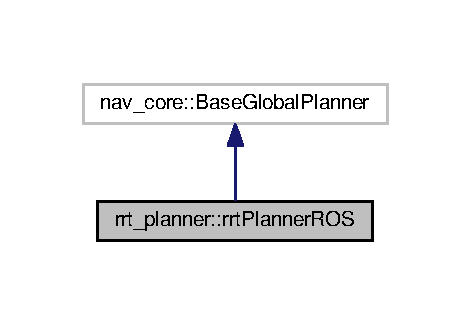
\includegraphics[width=226pt]{classrrt__planner_1_1rrtPlannerROS__inherit__graph}
\end{center}
\end{figure}


Collaboration diagram for rrt\+\_\+planner\+:\+:rrt\+Planner\+R\+OS\+:
\nopagebreak
\begin{figure}[H]
\begin{center}
\leavevmode
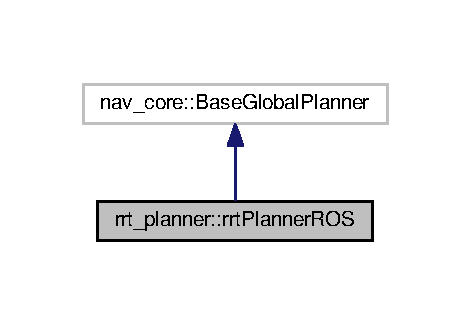
\includegraphics[width=226pt]{classrrt__planner_1_1rrtPlannerROS__coll__graph}
\end{center}
\end{figure}
\subsection*{Public Member Functions}
\begin{DoxyCompactItemize}
\item 
\hyperlink{classrrt__planner_1_1rrtPlannerROS_aa16e2cc2c0a27ef0a988d67d1d811bb5}{rrt\+Planner\+R\+OS} ()
\begin{DoxyCompactList}\small\item\em $<$ constructor \end{DoxyCompactList}\item 
\hyperlink{classrrt__planner_1_1rrtPlannerROS_af9bd26e4f73c143ff5016e30690476d2}{rrt\+Planner\+R\+OS} (std\+::string name, costmap\+\_\+2d\+::\+Costmap2\+D\+R\+OS $\ast$costmap\+\_\+ros)
\begin{DoxyCompactList}\small\item\em the node handler \end{DoxyCompactList}\item 
void \hyperlink{classrrt__planner_1_1rrtPlannerROS_ad58f8affe09327dc68321c37d1f123c3}{initialize} (std\+::string name, costmap\+\_\+2d\+::\+Costmap2\+D\+R\+OS $\ast$costmap\+\_\+ros)
\begin{DoxyCompactList}\small\item\em This function initialize the planner, and use the information provided by pgm/yaml map file. \end{DoxyCompactList}\item 
bool \hyperlink{classrrt__planner_1_1rrtPlannerROS_a753c96ea05471d2fc5710e883c6cbc3f}{make\+Plan} (const geometry\+\_\+msgs\+::\+Pose\+Stamped \&start, const geometry\+\_\+msgs\+::\+Pose\+Stamped \&goal, std\+::vector$<$ geometry\+\_\+msgs\+::\+Pose\+Stamped $>$ \&plan)
\begin{DoxyCompactList}\small\item\em This function works as the main function for calling planning algorithms. \end{DoxyCompactList}\item 
void \hyperlink{classrrt__planner_1_1rrtPlannerROS_a0765917723ac2e5cecdf526321bef3cb}{get\+Corrdinate} (float \&x, float \&y)
\begin{DoxyCompactList}\small\item\em This function does coordinate shift. \end{DoxyCompactList}\item 
int \hyperlink{classrrt__planner_1_1rrtPlannerROS_a92a01fb307538bf83e62c6f3b918fb99}{convert\+To\+Cell\+Index} (float x, float y)
\begin{DoxyCompactList}\small\item\em This function does coordinate transform whth a resolution to get the cell index. \end{DoxyCompactList}\item 
void \hyperlink{classrrt__planner_1_1rrtPlannerROS_adcb77afdad88d1d750b11582274b1a25}{convert\+To\+Coordinate} (int index, float \&x, float \&y)
\begin{DoxyCompactList}\small\item\em This function does coordinate transform. \end{DoxyCompactList}\item 
bool \hyperlink{classrrt__planner_1_1rrtPlannerROS_a0cb5c0fb53287fbee672088f57770eb2}{is\+Cell\+Inside\+Map} (float x, float y)
\begin{DoxyCompactList}\small\item\em check if the point is inside map \end{DoxyCompactList}\item 
std\+::vector$<$ int $>$ \hyperlink{classrrt__planner_1_1rrtPlannerROS_a8b0fecf1d9c07149b726e2983b01c44f}{rrt\+Planner} (int start\+Cell, int goal\+Cell)
\begin{DoxyCompactList}\small\item\em the core algorithm of rrt \end{DoxyCompactList}\item 
bool \hyperlink{classrrt__planner_1_1rrtPlannerROS_aee8b528868b043d60e740f909f463de6}{is\+Start\+And\+Goal\+Cells\+Valid} (int start\+Cell, int goal\+Cell)
\begin{DoxyCompactList}\small\item\em This function indicates if a start/goal point is valid. \end{DoxyCompactList}\item 
bool \hyperlink{classrrt__planner_1_1rrtPlannerROS_afda90bbd2bab0a0119346a5ac98bd274}{is\+Free} (int i, int j)
\begin{DoxyCompactList}\small\item\em This function indicates if a grid is occupied. \end{DoxyCompactList}\item 
bool \hyperlink{classrrt__planner_1_1rrtPlannerROS_a69ae9fe95e65fc3baa1e567ab33874a3}{is\+Free} (int Cell\+ID)
\begin{DoxyCompactList}\small\item\em This function indicates if a grid is occupied. \end{DoxyCompactList}\item 
std\+::pair$<$ int, int $>$ \hyperlink{classrrt__planner_1_1rrtPlannerROS_a06d1cb389e3ca07fb3b39173ce00c0a4}{Get\+Random\+Point} ()
\begin{DoxyCompactList}\small\item\em get a random point in the map \end{DoxyCompactList}\item 
int \hyperlink{classrrt__planner_1_1rrtPlannerROS_a047cc66d7055d8c39007c4de2db9ae59}{get\+Cell\+Index} (int i, int j)
\begin{DoxyCompactList}\small\item\em get the array index by the matrix coordinate \end{DoxyCompactList}\item 
int \hyperlink{classrrt__planner_1_1rrtPlannerROS_a77d03d9b7e48bd06504e318086b81339}{get\+Cell\+Row\+ID} (int index)
\begin{DoxyCompactList}\small\item\em get the row of the matrix coordinate by array index \end{DoxyCompactList}\item 
int \hyperlink{classrrt__planner_1_1rrtPlannerROS_ac2dfb825556d93e08c52c53142f0a081}{get\+Cell\+Col\+ID} (int index)
\begin{DoxyCompactList}\small\item\em get the col of the matrix coordinate by array index \end{DoxyCompactList}\end{DoxyCompactItemize}
\subsection*{Public Attributes}
\begin{DoxyCompactItemize}
\item 
ros\+::\+Node\+Handle \hyperlink{classrrt__planner_1_1rrtPlannerROS_ab0bceb51af7f6753d8ec3e5559b9bbb6}{R\+O\+S\+Node\+Handle}
\item 
int \hyperlink{classrrt__planner_1_1rrtPlannerROS_ae1f368fff6c8a74938f6283b22a035af}{width}
\item 
int \hyperlink{classrrt__planner_1_1rrtPlannerROS_ab8f1f1b80bc823050cdc9637830ff0bf}{height}
\item 
int \hyperlink{classrrt__planner_1_1rrtPlannerROS_a9d70e19d3be684a5df111ae5a3740b80}{map\+Size}
\item 
float \hyperlink{classrrt__planner_1_1rrtPlannerROS_a7937dc167bb0c96b33ca8e8287fef5bf}{resolution}
\begin{DoxyCompactList}\small\item\em the obstacle map \end{DoxyCompactList}\item 
bool $\ast$ \hyperlink{classrrt__planner_1_1rrtPlannerROS_a05a6e887d0cce7d410e25d151b30212c}{occupied\+Grid\+Map}
\begin{DoxyCompactList}\small\item\em the origin coordinate \end{DoxyCompactList}\item 
float \hyperlink{classrrt__planner_1_1rrtPlannerROS_a8788d318369f52f4fb20cacb9ea11b90}{originX}
\item 
float \hyperlink{classrrt__planner_1_1rrtPlannerROS_abd1ecbcdc24021b447f852abbefc6a87}{originY}
\begin{DoxyCompactList}\small\item\em the parameter of rrt algorithm \end{DoxyCompactList}\item 
double \hyperlink{classrrt__planner_1_1rrtPlannerROS_adf70aa722bdc79c72ebdfee4ce7bdce3}{step\+\_\+size\+\_\+}
\item 
double \hyperlink{classrrt__planner_1_1rrtPlannerROS_a969e711b8d5f06808309d80dda5b2326}{min\+\_\+dist\+\_\+from\+\_\+robot\+\_\+}
\item 
bool \hyperlink{classrrt__planner_1_1rrtPlannerROS_a5442c8d9c8e584229b9fb16eb53ee43e}{initialized\+\_\+}
\begin{DoxyCompactList}\small\item\em the map information \end{DoxyCompactList}\item 
costmap\+\_\+2d\+::\+Costmap2\+D\+R\+OS $\ast$ \hyperlink{classrrt__planner_1_1rrtPlannerROS_aab41b1ab3f521a762c1758ad3954cabd}{costmap\+\_\+ros\+\_\+}
\item 
costmap\+\_\+2d\+::\+Costmap2D $\ast$ \hyperlink{classrrt__planner_1_1rrtPlannerROS_a6a20af3d8a6b510429c39f2b64e31b8c}{costmap\+\_\+}
\end{DoxyCompactItemize}


\subsection{Constructor \& Destructor Documentation}
\index{rrt\+\_\+planner\+::rrt\+Planner\+R\+OS@{rrt\+\_\+planner\+::rrt\+Planner\+R\+OS}!rrt\+Planner\+R\+OS@{rrt\+Planner\+R\+OS}}
\index{rrt\+Planner\+R\+OS@{rrt\+Planner\+R\+OS}!rrt\+\_\+planner\+::rrt\+Planner\+R\+OS@{rrt\+\_\+planner\+::rrt\+Planner\+R\+OS}}
\subsubsection[{\texorpdfstring{rrt\+Planner\+R\+O\+S()}{rrtPlannerROS()}}]{\setlength{\rightskip}{0pt plus 5cm}rrt\+\_\+planner\+::rrt\+Planner\+R\+O\+S\+::rrt\+Planner\+R\+OS (
\begin{DoxyParamCaption}
{}
\end{DoxyParamCaption}
)}\hypertarget{classrrt__planner_1_1rrtPlannerROS_aa16e2cc2c0a27ef0a988d67d1d811bb5}{}\label{classrrt__planner_1_1rrtPlannerROS_aa16e2cc2c0a27ef0a988d67d1d811bb5}


$<$ constructor 

$<$ Constructors \index{rrt\+\_\+planner\+::rrt\+Planner\+R\+OS@{rrt\+\_\+planner\+::rrt\+Planner\+R\+OS}!rrt\+Planner\+R\+OS@{rrt\+Planner\+R\+OS}}
\index{rrt\+Planner\+R\+OS@{rrt\+Planner\+R\+OS}!rrt\+\_\+planner\+::rrt\+Planner\+R\+OS@{rrt\+\_\+planner\+::rrt\+Planner\+R\+OS}}
\subsubsection[{\texorpdfstring{rrt\+Planner\+R\+O\+S(std\+::string name, costmap\+\_\+2d\+::\+Costmap2\+D\+R\+O\+S $\ast$costmap\+\_\+ros)}{rrtPlannerROS(std::string name, costmap_2d::Costmap2DROS *costmap_ros)}}]{\setlength{\rightskip}{0pt plus 5cm}rrt\+\_\+planner\+::rrt\+Planner\+R\+O\+S\+::rrt\+Planner\+R\+OS (
\begin{DoxyParamCaption}
\item[{std\+::string}]{name, }
\item[{costmap\+\_\+2d\+::\+Costmap2\+D\+R\+OS $\ast$}]{costmap\+\_\+ros}
\end{DoxyParamCaption}
)}\hypertarget{classrrt__planner_1_1rrtPlannerROS_af9bd26e4f73c143ff5016e30690476d2}{}\label{classrrt__planner_1_1rrtPlannerROS_af9bd26e4f73c143ff5016e30690476d2}


the node handler 



\subsection{Member Function Documentation}
\index{rrt\+\_\+planner\+::rrt\+Planner\+R\+OS@{rrt\+\_\+planner\+::rrt\+Planner\+R\+OS}!convert\+To\+Cell\+Index@{convert\+To\+Cell\+Index}}
\index{convert\+To\+Cell\+Index@{convert\+To\+Cell\+Index}!rrt\+\_\+planner\+::rrt\+Planner\+R\+OS@{rrt\+\_\+planner\+::rrt\+Planner\+R\+OS}}
\subsubsection[{\texorpdfstring{convert\+To\+Cell\+Index(float x, float y)}{convertToCellIndex(float x, float y)}}]{\setlength{\rightskip}{0pt plus 5cm}int rrt\+\_\+planner\+::rrt\+Planner\+R\+O\+S\+::convert\+To\+Cell\+Index (
\begin{DoxyParamCaption}
\item[{float}]{x, }
\item[{float}]{y}
\end{DoxyParamCaption}
)}\hypertarget{classrrt__planner_1_1rrtPlannerROS_a92a01fb307538bf83e62c6f3b918fb99}{}\label{classrrt__planner_1_1rrtPlannerROS_a92a01fb307538bf83e62c6f3b918fb99}


This function does coordinate transform whth a resolution to get the cell index. 


\begin{DoxyParams}{Parameters}
{\em (x,y)} & \\
\hline
\end{DoxyParams}
\begin{DoxyReturn}{Returns}
int 
\end{DoxyReturn}
\index{rrt\+\_\+planner\+::rrt\+Planner\+R\+OS@{rrt\+\_\+planner\+::rrt\+Planner\+R\+OS}!convert\+To\+Coordinate@{convert\+To\+Coordinate}}
\index{convert\+To\+Coordinate@{convert\+To\+Coordinate}!rrt\+\_\+planner\+::rrt\+Planner\+R\+OS@{rrt\+\_\+planner\+::rrt\+Planner\+R\+OS}}
\subsubsection[{\texorpdfstring{convert\+To\+Coordinate(int index, float \&x, float \&y)}{convertToCoordinate(int index, float &x, float &y)}}]{\setlength{\rightskip}{0pt plus 5cm}void rrt\+\_\+planner\+::rrt\+Planner\+R\+O\+S\+::convert\+To\+Coordinate (
\begin{DoxyParamCaption}
\item[{int}]{index, }
\item[{float \&}]{x, }
\item[{float \&}]{y}
\end{DoxyParamCaption}
)}\hypertarget{classrrt__planner_1_1rrtPlannerROS_adcb77afdad88d1d750b11582274b1a25}{}\label{classrrt__planner_1_1rrtPlannerROS_adcb77afdad88d1d750b11582274b1a25}


This function does coordinate transform. 


\begin{DoxyParams}{Parameters}
{\em (index,x,y)} & \\
\hline
\end{DoxyParams}
\begin{DoxyReturn}{Returns}
void 
\end{DoxyReturn}
\index{rrt\+\_\+planner\+::rrt\+Planner\+R\+OS@{rrt\+\_\+planner\+::rrt\+Planner\+R\+OS}!get\+Cell\+Col\+ID@{get\+Cell\+Col\+ID}}
\index{get\+Cell\+Col\+ID@{get\+Cell\+Col\+ID}!rrt\+\_\+planner\+::rrt\+Planner\+R\+OS@{rrt\+\_\+planner\+::rrt\+Planner\+R\+OS}}
\subsubsection[{\texorpdfstring{get\+Cell\+Col\+I\+D(int index)}{getCellColID(int index)}}]{\setlength{\rightskip}{0pt plus 5cm}int rrt\+\_\+planner\+::rrt\+Planner\+R\+O\+S\+::get\+Cell\+Col\+ID (
\begin{DoxyParamCaption}
\item[{int}]{index}
\end{DoxyParamCaption}
)}\hypertarget{classrrt__planner_1_1rrtPlannerROS_ac2dfb825556d93e08c52c53142f0a081}{}\label{classrrt__planner_1_1rrtPlannerROS_ac2dfb825556d93e08c52c53142f0a081}


get the col of the matrix coordinate by array index 


\begin{DoxyParams}{Parameters}
{\em index} & \\
\hline
\end{DoxyParams}
\begin{DoxyReturn}{Returns}
col of the matrix 
\end{DoxyReturn}
\index{rrt\+\_\+planner\+::rrt\+Planner\+R\+OS@{rrt\+\_\+planner\+::rrt\+Planner\+R\+OS}!get\+Cell\+Index@{get\+Cell\+Index}}
\index{get\+Cell\+Index@{get\+Cell\+Index}!rrt\+\_\+planner\+::rrt\+Planner\+R\+OS@{rrt\+\_\+planner\+::rrt\+Planner\+R\+OS}}
\subsubsection[{\texorpdfstring{get\+Cell\+Index(int i, int j)}{getCellIndex(int i, int j)}}]{\setlength{\rightskip}{0pt plus 5cm}int rrt\+\_\+planner\+::rrt\+Planner\+R\+O\+S\+::get\+Cell\+Index (
\begin{DoxyParamCaption}
\item[{int}]{i, }
\item[{int}]{j}
\end{DoxyParamCaption}
)}\hypertarget{classrrt__planner_1_1rrtPlannerROS_a047cc66d7055d8c39007c4de2db9ae59}{}\label{classrrt__planner_1_1rrtPlannerROS_a047cc66d7055d8c39007c4de2db9ae59}


get the array index by the matrix coordinate 


\begin{DoxyParams}{Parameters}
{\em (i,j)} & \\
\hline
\end{DoxyParams}
\begin{DoxyReturn}{Returns}
the index of the array 
\end{DoxyReturn}
\index{rrt\+\_\+planner\+::rrt\+Planner\+R\+OS@{rrt\+\_\+planner\+::rrt\+Planner\+R\+OS}!get\+Cell\+Row\+ID@{get\+Cell\+Row\+ID}}
\index{get\+Cell\+Row\+ID@{get\+Cell\+Row\+ID}!rrt\+\_\+planner\+::rrt\+Planner\+R\+OS@{rrt\+\_\+planner\+::rrt\+Planner\+R\+OS}}
\subsubsection[{\texorpdfstring{get\+Cell\+Row\+I\+D(int index)}{getCellRowID(int index)}}]{\setlength{\rightskip}{0pt plus 5cm}int rrt\+\_\+planner\+::rrt\+Planner\+R\+O\+S\+::get\+Cell\+Row\+ID (
\begin{DoxyParamCaption}
\item[{int}]{index}
\end{DoxyParamCaption}
)}\hypertarget{classrrt__planner_1_1rrtPlannerROS_a77d03d9b7e48bd06504e318086b81339}{}\label{classrrt__planner_1_1rrtPlannerROS_a77d03d9b7e48bd06504e318086b81339}


get the row of the matrix coordinate by array index 


\begin{DoxyParams}{Parameters}
{\em index} & \\
\hline
\end{DoxyParams}
\begin{DoxyReturn}{Returns}
row of the matrix 
\end{DoxyReturn}
\index{rrt\+\_\+planner\+::rrt\+Planner\+R\+OS@{rrt\+\_\+planner\+::rrt\+Planner\+R\+OS}!get\+Corrdinate@{get\+Corrdinate}}
\index{get\+Corrdinate@{get\+Corrdinate}!rrt\+\_\+planner\+::rrt\+Planner\+R\+OS@{rrt\+\_\+planner\+::rrt\+Planner\+R\+OS}}
\subsubsection[{\texorpdfstring{get\+Corrdinate(float \&x, float \&y)}{getCorrdinate(float &x, float &y)}}]{\setlength{\rightskip}{0pt plus 5cm}void rrt\+\_\+planner\+::rrt\+Planner\+R\+O\+S\+::get\+Corrdinate (
\begin{DoxyParamCaption}
\item[{float \&}]{x, }
\item[{float \&}]{y}
\end{DoxyParamCaption}
)}\hypertarget{classrrt__planner_1_1rrtPlannerROS_a0765917723ac2e5cecdf526321bef3cb}{}\label{classrrt__planner_1_1rrtPlannerROS_a0765917723ac2e5cecdf526321bef3cb}


This function does coordinate shift. 


\begin{DoxyParams}{Parameters}
{\em (x,y)} & \\
\hline
\end{DoxyParams}
\begin{DoxyReturn}{Returns}
void 
\end{DoxyReturn}
\index{rrt\+\_\+planner\+::rrt\+Planner\+R\+OS@{rrt\+\_\+planner\+::rrt\+Planner\+R\+OS}!Get\+Random\+Point@{Get\+Random\+Point}}
\index{Get\+Random\+Point@{Get\+Random\+Point}!rrt\+\_\+planner\+::rrt\+Planner\+R\+OS@{rrt\+\_\+planner\+::rrt\+Planner\+R\+OS}}
\subsubsection[{\texorpdfstring{Get\+Random\+Point()}{GetRandomPoint()}}]{\setlength{\rightskip}{0pt plus 5cm}std\+::pair$<$ int, int $>$ rrt\+\_\+planner\+::rrt\+Planner\+R\+O\+S\+::\+Get\+Random\+Point (
\begin{DoxyParamCaption}
{}
\end{DoxyParamCaption}
)}\hypertarget{classrrt__planner_1_1rrtPlannerROS_a06d1cb389e3ca07fb3b39173ce00c0a4}{}\label{classrrt__planner_1_1rrtPlannerROS_a06d1cb389e3ca07fb3b39173ce00c0a4}


get a random point in the map 


\begin{DoxyParams}{Parameters}
{\em void} & \\
\hline
\end{DoxyParams}
\begin{DoxyReturn}{Returns}
pair$<$int, int$>$ 
\end{DoxyReturn}
\index{rrt\+\_\+planner\+::rrt\+Planner\+R\+OS@{rrt\+\_\+planner\+::rrt\+Planner\+R\+OS}!initialize@{initialize}}
\index{initialize@{initialize}!rrt\+\_\+planner\+::rrt\+Planner\+R\+OS@{rrt\+\_\+planner\+::rrt\+Planner\+R\+OS}}
\subsubsection[{\texorpdfstring{initialize(std\+::string name, costmap\+\_\+2d\+::\+Costmap2\+D\+R\+O\+S $\ast$costmap\+\_\+ros)}{initialize(std::string name, costmap_2d::Costmap2DROS *costmap_ros)}}]{\setlength{\rightskip}{0pt plus 5cm}void rrt\+\_\+planner\+::rrt\+Planner\+R\+O\+S\+::initialize (
\begin{DoxyParamCaption}
\item[{std\+::string}]{name, }
\item[{costmap\+\_\+2d\+::\+Costmap2\+D\+R\+OS $\ast$}]{costmap\+\_\+ros}
\end{DoxyParamCaption}
)}\hypertarget{classrrt__planner_1_1rrtPlannerROS_ad58f8affe09327dc68321c37d1f123c3}{}\label{classrrt__planner_1_1rrtPlannerROS_ad58f8affe09327dc68321c37d1f123c3}


This function initialize the planner, and use the information provided by pgm/yaml map file. 


\begin{DoxyParams}{Parameters}
{\em name,costmap\+\_\+ros} & \\
\hline
\end{DoxyParams}
\begin{DoxyReturn}{Returns}
none 
\end{DoxyReturn}
$<$ read the information from the map

$<$ build the occupied\+Grid\+Map with the given map \index{rrt\+\_\+planner\+::rrt\+Planner\+R\+OS@{rrt\+\_\+planner\+::rrt\+Planner\+R\+OS}!is\+Cell\+Inside\+Map@{is\+Cell\+Inside\+Map}}
\index{is\+Cell\+Inside\+Map@{is\+Cell\+Inside\+Map}!rrt\+\_\+planner\+::rrt\+Planner\+R\+OS@{rrt\+\_\+planner\+::rrt\+Planner\+R\+OS}}
\subsubsection[{\texorpdfstring{is\+Cell\+Inside\+Map(float x, float y)}{isCellInsideMap(float x, float y)}}]{\setlength{\rightskip}{0pt plus 5cm}bool rrt\+\_\+planner\+::rrt\+Planner\+R\+O\+S\+::is\+Cell\+Inside\+Map (
\begin{DoxyParamCaption}
\item[{float}]{x, }
\item[{float}]{y}
\end{DoxyParamCaption}
)}\hypertarget{classrrt__planner_1_1rrtPlannerROS_a0cb5c0fb53287fbee672088f57770eb2}{}\label{classrrt__planner_1_1rrtPlannerROS_a0cb5c0fb53287fbee672088f57770eb2}


check if the point is inside map 


\begin{DoxyParams}{Parameters}
{\em (x,y)} & \\
\hline
\end{DoxyParams}
\begin{DoxyReturn}{Returns}
bool 
\end{DoxyReturn}
\index{rrt\+\_\+planner\+::rrt\+Planner\+R\+OS@{rrt\+\_\+planner\+::rrt\+Planner\+R\+OS}!is\+Free@{is\+Free}}
\index{is\+Free@{is\+Free}!rrt\+\_\+planner\+::rrt\+Planner\+R\+OS@{rrt\+\_\+planner\+::rrt\+Planner\+R\+OS}}
\subsubsection[{\texorpdfstring{is\+Free(int i, int j)}{isFree(int i, int j)}}]{\setlength{\rightskip}{0pt plus 5cm}bool rrt\+\_\+planner\+::rrt\+Planner\+R\+O\+S\+::is\+Free (
\begin{DoxyParamCaption}
\item[{int}]{i, }
\item[{int}]{j}
\end{DoxyParamCaption}
)}\hypertarget{classrrt__planner_1_1rrtPlannerROS_afda90bbd2bab0a0119346a5ac98bd274}{}\label{classrrt__planner_1_1rrtPlannerROS_afda90bbd2bab0a0119346a5ac98bd274}


This function indicates if a grid is occupied. 


\begin{DoxyParams}{Parameters}
{\em (i,j),the} & coordinate of the occupied\+Grid\+Map \\
\hline
\end{DoxyParams}
\begin{DoxyReturn}{Returns}
if the cell is free 
\end{DoxyReturn}
\index{rrt\+\_\+planner\+::rrt\+Planner\+R\+OS@{rrt\+\_\+planner\+::rrt\+Planner\+R\+OS}!is\+Free@{is\+Free}}
\index{is\+Free@{is\+Free}!rrt\+\_\+planner\+::rrt\+Planner\+R\+OS@{rrt\+\_\+planner\+::rrt\+Planner\+R\+OS}}
\subsubsection[{\texorpdfstring{is\+Free(int Cell\+I\+D)}{isFree(int CellID)}}]{\setlength{\rightskip}{0pt plus 5cm}bool rrt\+\_\+planner\+::rrt\+Planner\+R\+O\+S\+::is\+Free (
\begin{DoxyParamCaption}
\item[{int}]{Cell\+ID}
\end{DoxyParamCaption}
)}\hypertarget{classrrt__planner_1_1rrtPlannerROS_a69ae9fe95e65fc3baa1e567ab33874a3}{}\label{classrrt__planner_1_1rrtPlannerROS_a69ae9fe95e65fc3baa1e567ab33874a3}


This function indicates if a grid is occupied. 


\begin{DoxyParams}{Parameters}
{\em Cell\+ID,the} & index of the occupied\+Grid\+Map \\
\hline
\end{DoxyParams}
\begin{DoxyReturn}{Returns}
if the cell is free 
\end{DoxyReturn}
\index{rrt\+\_\+planner\+::rrt\+Planner\+R\+OS@{rrt\+\_\+planner\+::rrt\+Planner\+R\+OS}!is\+Start\+And\+Goal\+Cells\+Valid@{is\+Start\+And\+Goal\+Cells\+Valid}}
\index{is\+Start\+And\+Goal\+Cells\+Valid@{is\+Start\+And\+Goal\+Cells\+Valid}!rrt\+\_\+planner\+::rrt\+Planner\+R\+OS@{rrt\+\_\+planner\+::rrt\+Planner\+R\+OS}}
\subsubsection[{\texorpdfstring{is\+Start\+And\+Goal\+Cells\+Valid(int start\+Cell, int goal\+Cell)}{isStartAndGoalCellsValid(int startCell, int goalCell)}}]{\setlength{\rightskip}{0pt plus 5cm}bool rrt\+\_\+planner\+::rrt\+Planner\+R\+O\+S\+::is\+Start\+And\+Goal\+Cells\+Valid (
\begin{DoxyParamCaption}
\item[{int}]{start\+Cell, }
\item[{int}]{goal\+Cell}
\end{DoxyParamCaption}
)}\hypertarget{classrrt__planner_1_1rrtPlannerROS_aee8b528868b043d60e740f909f463de6}{}\label{classrrt__planner_1_1rrtPlannerROS_aee8b528868b043d60e740f909f463de6}


This function indicates if a start/goal point is valid. 


\begin{DoxyParams}{Parameters}
{\em start\+Cell/goal\+Cell,the} & index of the occupied\+Grid\+Map \\
\hline
\end{DoxyParams}
\begin{DoxyReturn}{Returns}
if the cell is free 
\end{DoxyReturn}
\index{rrt\+\_\+planner\+::rrt\+Planner\+R\+OS@{rrt\+\_\+planner\+::rrt\+Planner\+R\+OS}!make\+Plan@{make\+Plan}}
\index{make\+Plan@{make\+Plan}!rrt\+\_\+planner\+::rrt\+Planner\+R\+OS@{rrt\+\_\+planner\+::rrt\+Planner\+R\+OS}}
\subsubsection[{\texorpdfstring{make\+Plan(const geometry\+\_\+msgs\+::\+Pose\+Stamped \&start, const geometry\+\_\+msgs\+::\+Pose\+Stamped \&goal, std\+::vector$<$ geometry\+\_\+msgs\+::\+Pose\+Stamped $>$ \&plan)}{makePlan(const geometry_msgs::PoseStamped &start, const geometry_msgs::PoseStamped &goal, std::vector< geometry_msgs::PoseStamped > &plan)}}]{\setlength{\rightskip}{0pt plus 5cm}bool rrt\+\_\+planner\+::rrt\+Planner\+R\+O\+S\+::make\+Plan (
\begin{DoxyParamCaption}
\item[{const geometry\+\_\+msgs\+::\+Pose\+Stamped \&}]{start, }
\item[{const geometry\+\_\+msgs\+::\+Pose\+Stamped \&}]{goal, }
\item[{std\+::vector$<$ geometry\+\_\+msgs\+::\+Pose\+Stamped $>$ \&}]{plan}
\end{DoxyParamCaption}
)}\hypertarget{classrrt__planner_1_1rrtPlannerROS_a753c96ea05471d2fc5710e883c6cbc3f}{}\label{classrrt__planner_1_1rrtPlannerROS_a753c96ea05471d2fc5710e883c6cbc3f}


This function works as the main function for calling planning algorithms. 


\begin{DoxyParams}{Parameters}
{\em start,goal,plan} & \\
\hline
\end{DoxyParams}
\begin{DoxyReturn}{Returns}
boolmatrix information 
\end{DoxyReturn}
$<$ change the coordinate of the position.

$<$ get the cell number of start/goal

$<$ start planning

$<$ if the global planner find a path

$<$ convert the path

$<$ convert the point to a \char`\"{}pose\char`\"{} \index{rrt\+\_\+planner\+::rrt\+Planner\+R\+OS@{rrt\+\_\+planner\+::rrt\+Planner\+R\+OS}!rrt\+Planner@{rrt\+Planner}}
\index{rrt\+Planner@{rrt\+Planner}!rrt\+\_\+planner\+::rrt\+Planner\+R\+OS@{rrt\+\_\+planner\+::rrt\+Planner\+R\+OS}}
\subsubsection[{\texorpdfstring{rrt\+Planner(int start\+Cell, int goal\+Cell)}{rrtPlanner(int startCell, int goalCell)}}]{\setlength{\rightskip}{0pt plus 5cm}std\+::vector$<$ int $>$ rrt\+\_\+planner\+::rrt\+Planner\+R\+O\+S\+::rrt\+Planner (
\begin{DoxyParamCaption}
\item[{int}]{start\+Cell, }
\item[{int}]{goal\+Cell}
\end{DoxyParamCaption}
)}\hypertarget{classrrt__planner_1_1rrtPlannerROS_a8b0fecf1d9c07149b726e2983b01c44f}{}\label{classrrt__planner_1_1rrtPlannerROS_a8b0fecf1d9c07149b726e2983b01c44f}


the core algorithm of rrt 


\begin{DoxyParams}{Parameters}
{\em start\+Cell,goal\+Cell} & \\
\hline
\end{DoxyParams}
\begin{DoxyReturn}{Returns}
std\+::vector$<$int$>$ 
\end{DoxyReturn}
$<$ start sampling

randomly choose a point in the map, with a small probability to choose the destination point

get the nearest vertex to the random point by iterating all the points in the search tree

build a new vertex along the direction\+: q\+\_\+near-\/$>$q\+\_\+rand q\+\_\+new is then added to the search tree.

$<$ if q\+\_\+new is valid, then save it to the search tree

$<$ check if the goal the goal found

$<$ use the destination as the initial point

$<$ sequentially put the path in a stack, the top is the start point 

\subsection{Member Data Documentation}
\index{rrt\+\_\+planner\+::rrt\+Planner\+R\+OS@{rrt\+\_\+planner\+::rrt\+Planner\+R\+OS}!costmap\+\_\+@{costmap\+\_\+}}
\index{costmap\+\_\+@{costmap\+\_\+}!rrt\+\_\+planner\+::rrt\+Planner\+R\+OS@{rrt\+\_\+planner\+::rrt\+Planner\+R\+OS}}
\subsubsection[{\texorpdfstring{costmap\+\_\+}{costmap_}}]{\setlength{\rightskip}{0pt plus 5cm}costmap\+\_\+2d\+::\+Costmap2D$\ast$ rrt\+\_\+planner\+::rrt\+Planner\+R\+O\+S\+::costmap\+\_\+}\hypertarget{classrrt__planner_1_1rrtPlannerROS_a6a20af3d8a6b510429c39f2b64e31b8c}{}\label{classrrt__planner_1_1rrtPlannerROS_a6a20af3d8a6b510429c39f2b64e31b8c}
\index{rrt\+\_\+planner\+::rrt\+Planner\+R\+OS@{rrt\+\_\+planner\+::rrt\+Planner\+R\+OS}!costmap\+\_\+ros\+\_\+@{costmap\+\_\+ros\+\_\+}}
\index{costmap\+\_\+ros\+\_\+@{costmap\+\_\+ros\+\_\+}!rrt\+\_\+planner\+::rrt\+Planner\+R\+OS@{rrt\+\_\+planner\+::rrt\+Planner\+R\+OS}}
\subsubsection[{\texorpdfstring{costmap\+\_\+ros\+\_\+}{costmap_ros_}}]{\setlength{\rightskip}{0pt plus 5cm}costmap\+\_\+2d\+::\+Costmap2\+D\+R\+OS$\ast$ rrt\+\_\+planner\+::rrt\+Planner\+R\+O\+S\+::costmap\+\_\+ros\+\_\+}\hypertarget{classrrt__planner_1_1rrtPlannerROS_aab41b1ab3f521a762c1758ad3954cabd}{}\label{classrrt__planner_1_1rrtPlannerROS_aab41b1ab3f521a762c1758ad3954cabd}
\index{rrt\+\_\+planner\+::rrt\+Planner\+R\+OS@{rrt\+\_\+planner\+::rrt\+Planner\+R\+OS}!height@{height}}
\index{height@{height}!rrt\+\_\+planner\+::rrt\+Planner\+R\+OS@{rrt\+\_\+planner\+::rrt\+Planner\+R\+OS}}
\subsubsection[{\texorpdfstring{height}{height}}]{\setlength{\rightskip}{0pt plus 5cm}int rrt\+\_\+planner\+::rrt\+Planner\+R\+O\+S\+::height}\hypertarget{classrrt__planner_1_1rrtPlannerROS_ab8f1f1b80bc823050cdc9637830ff0bf}{}\label{classrrt__planner_1_1rrtPlannerROS_ab8f1f1b80bc823050cdc9637830ff0bf}
\index{rrt\+\_\+planner\+::rrt\+Planner\+R\+OS@{rrt\+\_\+planner\+::rrt\+Planner\+R\+OS}!initialized\+\_\+@{initialized\+\_\+}}
\index{initialized\+\_\+@{initialized\+\_\+}!rrt\+\_\+planner\+::rrt\+Planner\+R\+OS@{rrt\+\_\+planner\+::rrt\+Planner\+R\+OS}}
\subsubsection[{\texorpdfstring{initialized\+\_\+}{initialized_}}]{\setlength{\rightskip}{0pt plus 5cm}bool rrt\+\_\+planner\+::rrt\+Planner\+R\+O\+S\+::initialized\+\_\+}\hypertarget{classrrt__planner_1_1rrtPlannerROS_a5442c8d9c8e584229b9fb16eb53ee43e}{}\label{classrrt__planner_1_1rrtPlannerROS_a5442c8d9c8e584229b9fb16eb53ee43e}


the map information 

\index{rrt\+\_\+planner\+::rrt\+Planner\+R\+OS@{rrt\+\_\+planner\+::rrt\+Planner\+R\+OS}!map\+Size@{map\+Size}}
\index{map\+Size@{map\+Size}!rrt\+\_\+planner\+::rrt\+Planner\+R\+OS@{rrt\+\_\+planner\+::rrt\+Planner\+R\+OS}}
\subsubsection[{\texorpdfstring{map\+Size}{mapSize}}]{\setlength{\rightskip}{0pt plus 5cm}int rrt\+\_\+planner\+::rrt\+Planner\+R\+O\+S\+::map\+Size}\hypertarget{classrrt__planner_1_1rrtPlannerROS_a9d70e19d3be684a5df111ae5a3740b80}{}\label{classrrt__planner_1_1rrtPlannerROS_a9d70e19d3be684a5df111ae5a3740b80}
\index{rrt\+\_\+planner\+::rrt\+Planner\+R\+OS@{rrt\+\_\+planner\+::rrt\+Planner\+R\+OS}!min\+\_\+dist\+\_\+from\+\_\+robot\+\_\+@{min\+\_\+dist\+\_\+from\+\_\+robot\+\_\+}}
\index{min\+\_\+dist\+\_\+from\+\_\+robot\+\_\+@{min\+\_\+dist\+\_\+from\+\_\+robot\+\_\+}!rrt\+\_\+planner\+::rrt\+Planner\+R\+OS@{rrt\+\_\+planner\+::rrt\+Planner\+R\+OS}}
\subsubsection[{\texorpdfstring{min\+\_\+dist\+\_\+from\+\_\+robot\+\_\+}{min_dist_from_robot_}}]{\setlength{\rightskip}{0pt plus 5cm}double rrt\+\_\+planner\+::rrt\+Planner\+R\+O\+S\+::min\+\_\+dist\+\_\+from\+\_\+robot\+\_\+}\hypertarget{classrrt__planner_1_1rrtPlannerROS_a969e711b8d5f06808309d80dda5b2326}{}\label{classrrt__planner_1_1rrtPlannerROS_a969e711b8d5f06808309d80dda5b2326}
\index{rrt\+\_\+planner\+::rrt\+Planner\+R\+OS@{rrt\+\_\+planner\+::rrt\+Planner\+R\+OS}!occupied\+Grid\+Map@{occupied\+Grid\+Map}}
\index{occupied\+Grid\+Map@{occupied\+Grid\+Map}!rrt\+\_\+planner\+::rrt\+Planner\+R\+OS@{rrt\+\_\+planner\+::rrt\+Planner\+R\+OS}}
\subsubsection[{\texorpdfstring{occupied\+Grid\+Map}{occupiedGridMap}}]{\setlength{\rightskip}{0pt plus 5cm}bool$\ast$ rrt\+\_\+planner\+::rrt\+Planner\+R\+O\+S\+::occupied\+Grid\+Map}\hypertarget{classrrt__planner_1_1rrtPlannerROS_a05a6e887d0cce7d410e25d151b30212c}{}\label{classrrt__planner_1_1rrtPlannerROS_a05a6e887d0cce7d410e25d151b30212c}


the origin coordinate 

\index{rrt\+\_\+planner\+::rrt\+Planner\+R\+OS@{rrt\+\_\+planner\+::rrt\+Planner\+R\+OS}!originX@{originX}}
\index{originX@{originX}!rrt\+\_\+planner\+::rrt\+Planner\+R\+OS@{rrt\+\_\+planner\+::rrt\+Planner\+R\+OS}}
\subsubsection[{\texorpdfstring{originX}{originX}}]{\setlength{\rightskip}{0pt plus 5cm}float rrt\+\_\+planner\+::rrt\+Planner\+R\+O\+S\+::originX}\hypertarget{classrrt__planner_1_1rrtPlannerROS_a8788d318369f52f4fb20cacb9ea11b90}{}\label{classrrt__planner_1_1rrtPlannerROS_a8788d318369f52f4fb20cacb9ea11b90}
\index{rrt\+\_\+planner\+::rrt\+Planner\+R\+OS@{rrt\+\_\+planner\+::rrt\+Planner\+R\+OS}!originY@{originY}}
\index{originY@{originY}!rrt\+\_\+planner\+::rrt\+Planner\+R\+OS@{rrt\+\_\+planner\+::rrt\+Planner\+R\+OS}}
\subsubsection[{\texorpdfstring{originY}{originY}}]{\setlength{\rightskip}{0pt plus 5cm}float rrt\+\_\+planner\+::rrt\+Planner\+R\+O\+S\+::originY}\hypertarget{classrrt__planner_1_1rrtPlannerROS_abd1ecbcdc24021b447f852abbefc6a87}{}\label{classrrt__planner_1_1rrtPlannerROS_abd1ecbcdc24021b447f852abbefc6a87}


the parameter of rrt algorithm 

\index{rrt\+\_\+planner\+::rrt\+Planner\+R\+OS@{rrt\+\_\+planner\+::rrt\+Planner\+R\+OS}!resolution@{resolution}}
\index{resolution@{resolution}!rrt\+\_\+planner\+::rrt\+Planner\+R\+OS@{rrt\+\_\+planner\+::rrt\+Planner\+R\+OS}}
\subsubsection[{\texorpdfstring{resolution}{resolution}}]{\setlength{\rightskip}{0pt plus 5cm}float rrt\+\_\+planner\+::rrt\+Planner\+R\+O\+S\+::resolution}\hypertarget{classrrt__planner_1_1rrtPlannerROS_a7937dc167bb0c96b33ca8e8287fef5bf}{}\label{classrrt__planner_1_1rrtPlannerROS_a7937dc167bb0c96b33ca8e8287fef5bf}


the obstacle map 

\index{rrt\+\_\+planner\+::rrt\+Planner\+R\+OS@{rrt\+\_\+planner\+::rrt\+Planner\+R\+OS}!R\+O\+S\+Node\+Handle@{R\+O\+S\+Node\+Handle}}
\index{R\+O\+S\+Node\+Handle@{R\+O\+S\+Node\+Handle}!rrt\+\_\+planner\+::rrt\+Planner\+R\+OS@{rrt\+\_\+planner\+::rrt\+Planner\+R\+OS}}
\subsubsection[{\texorpdfstring{R\+O\+S\+Node\+Handle}{ROSNodeHandle}}]{\setlength{\rightskip}{0pt plus 5cm}ros\+::\+Node\+Handle rrt\+\_\+planner\+::rrt\+Planner\+R\+O\+S\+::\+R\+O\+S\+Node\+Handle}\hypertarget{classrrt__planner_1_1rrtPlannerROS_ab0bceb51af7f6753d8ec3e5559b9bbb6}{}\label{classrrt__planner_1_1rrtPlannerROS_ab0bceb51af7f6753d8ec3e5559b9bbb6}
\index{rrt\+\_\+planner\+::rrt\+Planner\+R\+OS@{rrt\+\_\+planner\+::rrt\+Planner\+R\+OS}!step\+\_\+size\+\_\+@{step\+\_\+size\+\_\+}}
\index{step\+\_\+size\+\_\+@{step\+\_\+size\+\_\+}!rrt\+\_\+planner\+::rrt\+Planner\+R\+OS@{rrt\+\_\+planner\+::rrt\+Planner\+R\+OS}}
\subsubsection[{\texorpdfstring{step\+\_\+size\+\_\+}{step_size_}}]{\setlength{\rightskip}{0pt plus 5cm}double rrt\+\_\+planner\+::rrt\+Planner\+R\+O\+S\+::step\+\_\+size\+\_\+}\hypertarget{classrrt__planner_1_1rrtPlannerROS_adf70aa722bdc79c72ebdfee4ce7bdce3}{}\label{classrrt__planner_1_1rrtPlannerROS_adf70aa722bdc79c72ebdfee4ce7bdce3}
\index{rrt\+\_\+planner\+::rrt\+Planner\+R\+OS@{rrt\+\_\+planner\+::rrt\+Planner\+R\+OS}!width@{width}}
\index{width@{width}!rrt\+\_\+planner\+::rrt\+Planner\+R\+OS@{rrt\+\_\+planner\+::rrt\+Planner\+R\+OS}}
\subsubsection[{\texorpdfstring{width}{width}}]{\setlength{\rightskip}{0pt plus 5cm}int rrt\+\_\+planner\+::rrt\+Planner\+R\+O\+S\+::width}\hypertarget{classrrt__planner_1_1rrtPlannerROS_ae1f368fff6c8a74938f6283b22a035af}{}\label{classrrt__planner_1_1rrtPlannerROS_ae1f368fff6c8a74938f6283b22a035af}


The documentation for this class was generated from the following files\+:\begin{DoxyCompactItemize}
\item 
/home/cptsai/catkin\+\_\+ws/src/\+E\+N\+P\+M808\+X/\+R\+O\+S/\+Turtlebot\+\_\+\+R\+R\+T\+\_\+\+S\+L\+A\+M/include/\hyperlink{rrt__global__planner__plugin_8h}{rrt\+\_\+global\+\_\+planner\+\_\+plugin.\+h}\item 
/home/cptsai/catkin\+\_\+ws/src/\+E\+N\+P\+M808\+X/\+R\+O\+S/\+Turtlebot\+\_\+\+R\+R\+T\+\_\+\+S\+L\+A\+M/src/\hyperlink{rrt__global__planner__plugin_8cpp}{rrt\+\_\+global\+\_\+planner\+\_\+plugin.\+cpp}\end{DoxyCompactItemize}

\hypertarget{classvertex}{}\section{vertex Class Reference}
\label{classvertex}\index{vertex@{vertex}}


definition of a point in R\+RT  




{\ttfamily \#include $<$rrt\+\_\+global\+\_\+planner\+\_\+plugin.\+h$>$}

\subsection*{Public Member Functions}
\begin{DoxyCompactItemize}
\item 
void \hyperlink{classvertex_a6f60229a39cc2c87517d5da16737c0fe}{set\+Position} (float x, float y)
\begin{DoxyCompactList}\small\item\em $<$ set the coordinate of the vertex \end{DoxyCompactList}\item 
void \hyperlink{classvertex_a88b35e277467413154d64dceaffc26f7}{set\+Parent\+Idx} (int idx)
\begin{DoxyCompactList}\small\item\em set the index of the vertex \end{DoxyCompactList}\item 
void \hyperlink{classvertex_ac723537f91a75552cf98d53778327408}{set\+Idx} (int i)
\begin{DoxyCompactList}\small\item\em get the coordinate of the vertex \end{DoxyCompactList}\item 
std\+::pair$<$ float, float $>$ \hyperlink{classvertex_af3192c89865d850b2a656e2ee840907d}{get\+Position} ()
\begin{DoxyCompactList}\small\item\em get the parent index of the vertex \end{DoxyCompactList}\item 
int \hyperlink{classvertex_aa7d695c2874361b913447b79bc047814}{get\+Parent\+Idx} ()
\begin{DoxyCompactList}\small\item\em get the index of the vertex \end{DoxyCompactList}\item 
int \hyperlink{classvertex_ae21069e33ecfb0c5cb7c17befe1c3e60}{get\+Idx} ()
\begin{DoxyCompactList}\small\item\em class \hyperlink{namespacerrt__planner}{rrt\+\_\+planner} methods \end{DoxyCompactList}\end{DoxyCompactItemize}


\subsection{Detailed Description}
definition of a point in R\+RT 

\subsection{Member Function Documentation}
\index{vertex@{vertex}!get\+Idx@{get\+Idx}}
\index{get\+Idx@{get\+Idx}!vertex@{vertex}}
\subsubsection[{\texorpdfstring{get\+Idx()}{getIdx()}}]{\setlength{\rightskip}{0pt plus 5cm}int vertex\+::get\+Idx (
\begin{DoxyParamCaption}
{}
\end{DoxyParamCaption}
)}\hypertarget{classvertex_ae21069e33ecfb0c5cb7c17befe1c3e60}{}\label{classvertex_ae21069e33ecfb0c5cb7c17befe1c3e60}


class \hyperlink{namespacerrt__planner}{rrt\+\_\+planner} methods 

\index{vertex@{vertex}!get\+Parent\+Idx@{get\+Parent\+Idx}}
\index{get\+Parent\+Idx@{get\+Parent\+Idx}!vertex@{vertex}}
\subsubsection[{\texorpdfstring{get\+Parent\+Idx()}{getParentIdx()}}]{\setlength{\rightskip}{0pt plus 5cm}int vertex\+::get\+Parent\+Idx (
\begin{DoxyParamCaption}
{}
\end{DoxyParamCaption}
)}\hypertarget{classvertex_aa7d695c2874361b913447b79bc047814}{}\label{classvertex_aa7d695c2874361b913447b79bc047814}


get the index of the vertex 

\index{vertex@{vertex}!get\+Position@{get\+Position}}
\index{get\+Position@{get\+Position}!vertex@{vertex}}
\subsubsection[{\texorpdfstring{get\+Position()}{getPosition()}}]{\setlength{\rightskip}{0pt plus 5cm}std\+::pair$<$ float, float $>$ vertex\+::get\+Position (
\begin{DoxyParamCaption}
{}
\end{DoxyParamCaption}
)}\hypertarget{classvertex_af3192c89865d850b2a656e2ee840907d}{}\label{classvertex_af3192c89865d850b2a656e2ee840907d}


get the parent index of the vertex 

\index{vertex@{vertex}!set\+Idx@{set\+Idx}}
\index{set\+Idx@{set\+Idx}!vertex@{vertex}}
\subsubsection[{\texorpdfstring{set\+Idx(int i)}{setIdx(int i)}}]{\setlength{\rightskip}{0pt plus 5cm}void vertex\+::set\+Idx (
\begin{DoxyParamCaption}
\item[{int}]{i}
\end{DoxyParamCaption}
)}\hypertarget{classvertex_ac723537f91a75552cf98d53778327408}{}\label{classvertex_ac723537f91a75552cf98d53778327408}


get the coordinate of the vertex 

\index{vertex@{vertex}!set\+Parent\+Idx@{set\+Parent\+Idx}}
\index{set\+Parent\+Idx@{set\+Parent\+Idx}!vertex@{vertex}}
\subsubsection[{\texorpdfstring{set\+Parent\+Idx(int idx)}{setParentIdx(int idx)}}]{\setlength{\rightskip}{0pt plus 5cm}void vertex\+::set\+Parent\+Idx (
\begin{DoxyParamCaption}
\item[{int}]{idx}
\end{DoxyParamCaption}
)}\hypertarget{classvertex_a88b35e277467413154d64dceaffc26f7}{}\label{classvertex_a88b35e277467413154d64dceaffc26f7}


set the index of the vertex 

\index{vertex@{vertex}!set\+Position@{set\+Position}}
\index{set\+Position@{set\+Position}!vertex@{vertex}}
\subsubsection[{\texorpdfstring{set\+Position(float x, float y)}{setPosition(float x, float y)}}]{\setlength{\rightskip}{0pt plus 5cm}void vertex\+::set\+Position (
\begin{DoxyParamCaption}
\item[{float}]{x, }
\item[{float}]{y}
\end{DoxyParamCaption}
)}\hypertarget{classvertex_a6f60229a39cc2c87517d5da16737c0fe}{}\label{classvertex_a6f60229a39cc2c87517d5da16737c0fe}


$<$ set the coordinate of the vertex 

$<$ register this planner as a Base\+Global\+Planner plugin

set the parent index of the vertex

$<$ vertex function implementation 

The documentation for this class was generated from the following files\+:\begin{DoxyCompactItemize}
\item 
/home/cptsai/catkin\+\_\+ws/src/\+E\+N\+P\+M808\+X/\+R\+O\+S/\+Turtlebot\+\_\+\+R\+R\+T\+\_\+\+S\+L\+A\+M/include/\hyperlink{rrt__global__planner__plugin_8h}{rrt\+\_\+global\+\_\+planner\+\_\+plugin.\+h}\item 
/home/cptsai/catkin\+\_\+ws/src/\+E\+N\+P\+M808\+X/\+R\+O\+S/\+Turtlebot\+\_\+\+R\+R\+T\+\_\+\+S\+L\+A\+M/src/\hyperlink{rrt__global__planner__plugin_8cpp}{rrt\+\_\+global\+\_\+planner\+\_\+plugin.\+cpp}\end{DoxyCompactItemize}

\chapter{File Documentation}
\hypertarget{rrt__global__planner__plugin_8h}{}\section{/home/cptsai/catkin\+\_\+ws/src/\+E\+N\+P\+M808\+X/\+R\+O\+S/\+Turtlebot\+\_\+\+R\+R\+T\+\_\+\+S\+L\+A\+M/include/rrt\+\_\+global\+\_\+planner\+\_\+plugin.h File Reference}
\label{rrt__global__planner__plugin_8h}\index{/home/cptsai/catkin\+\_\+ws/src/\+E\+N\+P\+M808\+X/\+R\+O\+S/\+Turtlebot\+\_\+\+R\+R\+T\+\_\+\+S\+L\+A\+M/include/rrt\+\_\+global\+\_\+planner\+\_\+plugin.\+h@{/home/cptsai/catkin\+\_\+ws/src/\+E\+N\+P\+M808\+X/\+R\+O\+S/\+Turtlebot\+\_\+\+R\+R\+T\+\_\+\+S\+L\+A\+M/include/rrt\+\_\+global\+\_\+planner\+\_\+plugin.\+h}}


Definition of rrt global planner.  


{\ttfamily \#include $<$string.\+h$>$}\\*
{\ttfamily \#include $<$sys/types.\+h$>$}\\*
{\ttfamily \#include $<$sys/socket.\+h$>$}\\*
{\ttfamily \#include $<$netinet/in.\+h$>$}\\*
{\ttfamily \#include $<$netdb.\+h$>$}\\*
{\ttfamily \#include $<$ros/ros.\+h$>$}\\*
{\ttfamily \#include $<$actionlib/client/simple\+\_\+action\+\_\+client.\+h$>$}\\*
{\ttfamily \#include $<$move\+\_\+base\+\_\+msgs/\+Move\+Base\+Action.\+h$>$}\\*
{\ttfamily \#include $<$geometry\+\_\+msgs/\+Twist.\+h$>$}\\*
{\ttfamily \#include $<$angles/angles.\+h$>$}\\*
{\ttfamily \#include $<$base\+\_\+local\+\_\+planner/world\+\_\+model.\+h$>$}\\*
{\ttfamily \#include $<$base\+\_\+local\+\_\+planner/costmap\+\_\+model.\+h$>$}\\*
{\ttfamily \#include $<$nav\+\_\+core/base\+\_\+global\+\_\+planner.\+h$>$}\\*
{\ttfamily \#include $<$geometry\+\_\+msgs/\+Pose\+Stamped.\+h$>$}\\*
{\ttfamily \#include $<$costmap\+\_\+2d/costmap\+\_\+2d.\+h$>$}\\*
{\ttfamily \#include $<$costmap\+\_\+2d/costmap\+\_\+2d\+\_\+ros.\+h$>$}\\*
{\ttfamily \#include $<$nav\+\_\+msgs/\+Odometry.\+h$>$}\\*
{\ttfamily \#include $<$nav\+\_\+msgs/\+Occupancy\+Grid.\+h$>$}\\*
{\ttfamily \#include $<$nav\+\_\+msgs/\+Path.\+h$>$}\\*
{\ttfamily \#include $<$nav\+\_\+msgs/\+Get\+Plan.\+h$>$}\\*
{\ttfamily \#include $<$tf/tf.\+h$>$}\\*
{\ttfamily \#include $<$tf/transform\+\_\+datatypes.\+h$>$}\\*
{\ttfamily \#include $<$tf/transform\+\_\+listener.\+h$>$}\\*
{\ttfamily \#include $<$stdio.\+h$>$}\\*
{\ttfamily \#include $<$stdlib.\+h$>$}\\*
{\ttfamily \#include $<$unistd.\+h$>$}\\*
{\ttfamily \#include $<$geometry\+\_\+msgs/\+Pose\+With\+Covariance\+Stamped.\+h$>$}\\*
{\ttfamily \#include $<$move\+\_\+base\+\_\+msgs/\+Move\+Base\+Goal.\+h$>$}\\*
{\ttfamily \#include $<$move\+\_\+base\+\_\+msgs/\+Move\+Base\+Action\+Goal.\+h$>$}\\*
{\ttfamily \#include $<$set$>$}\\*
{\ttfamily \#include $<$string$>$}\\*
{\ttfamily \#include $<$vector$>$}\\*
{\ttfamily \#include $<$utility$>$}\\*
{\ttfamily \#include $<$random$>$}\\*
{\ttfamily \#include \char`\"{}sensor\+\_\+msgs/\+Laser\+Scan.\+h\char`\"{}}\\*
{\ttfamily \#include \char`\"{}sensor\+\_\+msgs/\+Point\+Cloud2.\+h\char`\"{}}\\*
{\ttfamily \#include $<$boost/foreach.\+hpp$>$}\\*
Include dependency graph for rrt\+\_\+global\+\_\+planner\+\_\+plugin.\+h\+:
\nopagebreak
\begin{figure}[H]
\begin{center}
\leavevmode
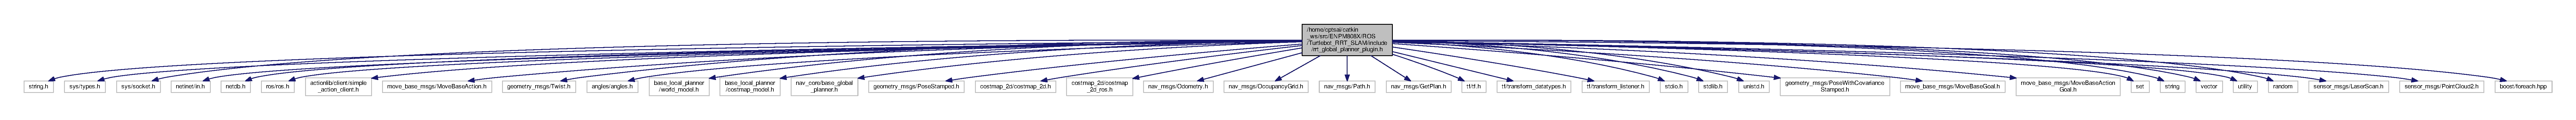
\includegraphics[width=350pt]{rrt__global__planner__plugin_8h__incl}
\end{center}
\end{figure}
This graph shows which files directly or indirectly include this file\+:
\nopagebreak
\begin{figure}[H]
\begin{center}
\leavevmode
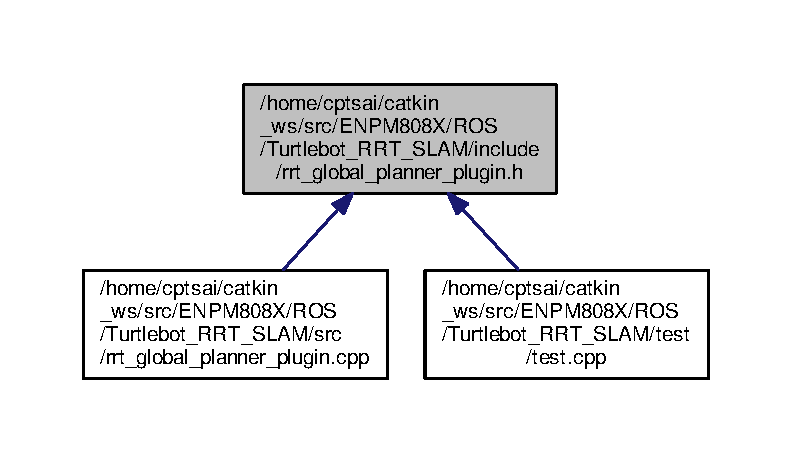
\includegraphics[width=350pt]{rrt__global__planner__plugin_8h__dep__incl}
\end{center}
\end{figure}
\subsection*{Classes}
\begin{DoxyCompactItemize}
\item 
class \hyperlink{classvertex}{vertex}
\begin{DoxyCompactList}\small\item\em definition of a point in R\+RT \end{DoxyCompactList}\item 
class \hyperlink{classrrt__planner_1_1rrtPlannerROS}{rrt\+\_\+planner\+::rrt\+Planner\+R\+OS}
\end{DoxyCompactItemize}
\subsection*{Namespaces}
\begin{DoxyCompactItemize}
\item 
 \hyperlink{namespacerrt__planner}{rrt\+\_\+planner}
\end{DoxyCompactItemize}


\subsection{Detailed Description}
Definition of rrt global planner. 

B\+SD License Copyright $<$2018$>$ $<$Chien-\/\+Te Lee$>$ $<$Chin-\/\+Po Tsai$>$

Redistribution and use in source and binary forms, with or without modification, are permitted provided that the following conditions are met\+:


\begin{DoxyEnumerate}
\item Redistributions of source code must retain the above copyright notice, this list of conditions and the following disclaimer.
\item Redistributions in binary form must reproduce the above copyright notice, this list of conditions and the following disclaimer in the documentation and/or other materials provided with the distribution.
\item Neither the name of the copyright holder nor the names of its contributors may be used to endorse or promote products derived from this software without specific prior written permission.
\end{DoxyEnumerate}

T\+H\+IS S\+O\+F\+T\+W\+A\+RE IS P\+R\+O\+V\+I\+D\+ED BY T\+HE C\+O\+P\+Y\+R\+I\+G\+HT H\+O\+L\+D\+E\+RS A\+ND C\+O\+N\+T\+R\+I\+B\+U\+T\+O\+RS \char`\"{}\+A\+S I\+S\char`\"{} A\+ND A\+NY E\+X\+P\+R\+E\+SS OR I\+M\+P\+L\+I\+ED W\+A\+R\+R\+A\+N\+T\+I\+ES, I\+N\+C\+L\+U\+D\+I\+NG, B\+UT N\+OT L\+I\+M\+I\+T\+ED TO, T\+HE I\+M\+P\+L\+I\+ED W\+A\+R\+R\+A\+N\+T\+I\+ES OF M\+E\+R\+C\+H\+A\+N\+T\+A\+B\+I\+L\+I\+TY A\+ND F\+I\+T\+N\+E\+SS F\+OR A P\+A\+R\+T\+I\+C\+U\+L\+AR P\+U\+R\+P\+O\+SE A\+RE D\+I\+S\+C\+L\+A\+I\+M\+ED. IN NO E\+V\+E\+NT S\+H\+A\+LL T\+HE C\+O\+P\+Y\+R\+I\+G\+HT H\+O\+L\+D\+ER OR C\+O\+N\+T\+R\+I\+B\+U\+T\+O\+RS BE L\+I\+A\+B\+LE F\+OR A\+NY D\+I\+R\+E\+CT, I\+N\+D\+I\+R\+E\+CT, I\+N\+C\+I\+D\+E\+N\+T\+AL, S\+P\+E\+C\+I\+AL, E\+X\+E\+M\+P\+L\+A\+RY, OR C\+O\+N\+S\+E\+Q\+U\+E\+N\+T\+I\+AL D\+A\+M\+A\+G\+ES (I\+N\+C\+L\+U\+D\+I\+NG, B\+UT N\+OT L\+I\+M\+I\+T\+ED TO, P\+R\+O\+C\+U\+R\+E\+M\+E\+NT OF S\+U\+B\+S\+T\+I\+T\+U\+TE G\+O\+O\+DS OR S\+E\+R\+V\+I\+C\+ES; L\+O\+SS OF U\+SE, D\+A\+TA, OR P\+R\+O\+F\+I\+TS; OR B\+U\+S\+I\+N\+E\+SS I\+N\+T\+E\+R\+R\+U\+P\+T\+I\+ON) H\+O\+W\+E\+V\+ER C\+A\+U\+S\+ED A\+ND ON A\+NY T\+H\+E\+O\+RY OF L\+I\+A\+B\+I\+L\+I\+TY, W\+H\+E\+T\+H\+ER IN C\+O\+N\+T\+R\+A\+CT, S\+T\+R\+I\+CT L\+I\+A\+B\+I\+L\+I\+TY, OR T\+O\+RT (I\+N\+C\+L\+U\+D\+I\+NG N\+E\+G\+L\+I\+G\+E\+N\+CE OR O\+T\+H\+E\+R\+W\+I\+SE) A\+R\+I\+S\+I\+NG IN A\+NY W\+AY O\+UT OF T\+HE U\+SE OF T\+H\+IS S\+O\+F\+T\+W\+A\+RE, E\+V\+EN IF A\+D\+V\+I\+S\+ED OF T\+HE P\+O\+S\+S\+I\+B\+I\+L\+I\+TY OF S\+U\+CH D\+A\+M\+A\+GE. \begin{DoxyCopyright}{Copyright}
(c) 2018 Chien-\/\+Te Lee, Chin-\/\+Po Tsai 
\end{DoxyCopyright}
\begin{DoxyAuthor}{Author}
Chien-\/\+Te Lee, Chin-\/\+Po Tsai 
\end{DoxyAuthor}
\begin{DoxyDate}{Date}
12/12/2018
\end{DoxyDate}
This file is the definition for rrt 
\hypertarget{twist__to__wheel_8h}{}\section{/home/cptsai/catkin\+\_\+ws/src/\+E\+N\+P\+M808\+X/\+R\+O\+S/\+Turtlebot\+\_\+\+R\+R\+T\+\_\+\+S\+L\+A\+M/include/twist\+\_\+to\+\_\+wheel.h File Reference}
\label{twist__to__wheel_8h}\index{/home/cptsai/catkin\+\_\+ws/src/\+E\+N\+P\+M808\+X/\+R\+O\+S/\+Turtlebot\+\_\+\+R\+R\+T\+\_\+\+S\+L\+A\+M/include/twist\+\_\+to\+\_\+wheel.\+h@{/home/cptsai/catkin\+\_\+ws/src/\+E\+N\+P\+M808\+X/\+R\+O\+S/\+Turtlebot\+\_\+\+R\+R\+T\+\_\+\+S\+L\+A\+M/include/twist\+\_\+to\+\_\+wheel.\+h}}


Definition of twist\+\_\+to\+\_\+wheel call back function.  


{\ttfamily \#include $<$ros/ros.\+h$>$}\\*
{\ttfamily \#include $<$tf/transform\+\_\+listener.\+h$>$}\\*
{\ttfamily \#include $<$geometry\+\_\+msgs/\+Twist.\+h$>$}\\*
Include dependency graph for twist\+\_\+to\+\_\+wheel.\+h\+:
\nopagebreak
\begin{figure}[H]
\begin{center}
\leavevmode
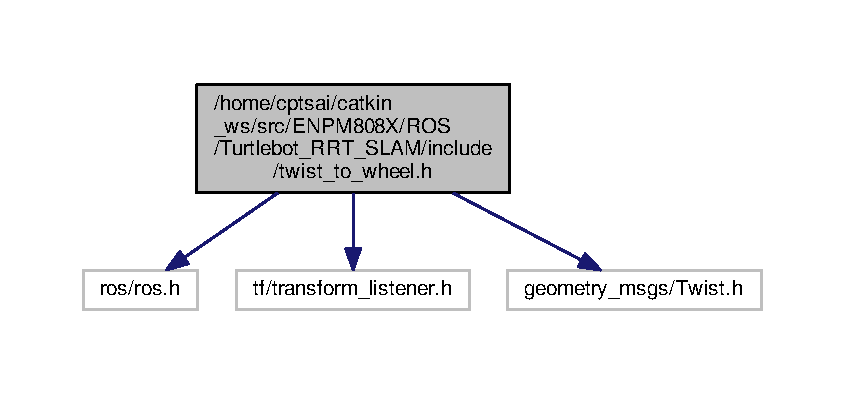
\includegraphics[width=350pt]{twist__to__wheel_8h__incl}
\end{center}
\end{figure}
This graph shows which files directly or indirectly include this file\+:
\nopagebreak
\begin{figure}[H]
\begin{center}
\leavevmode
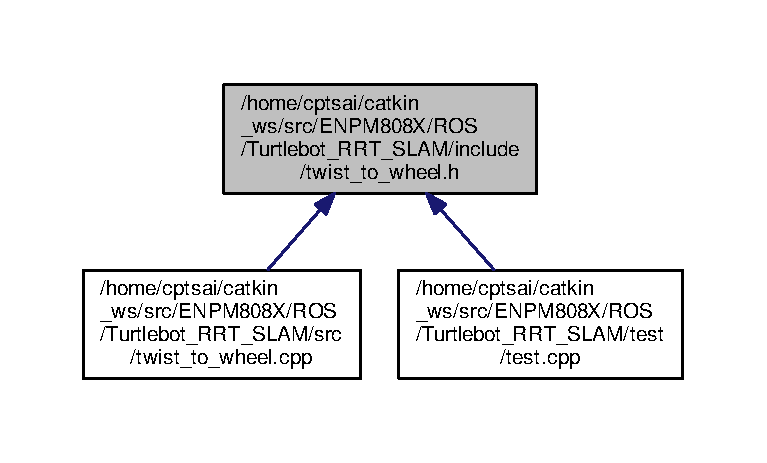
\includegraphics[width=350pt]{twist__to__wheel_8h__dep__incl}
\end{center}
\end{figure}
\subsection*{Functions}
\begin{DoxyCompactItemize}
\item 
void \hyperlink{twist__to__wheel_8h_adc7cb856e4fa79127a024420e18e6096}{twist\+Cb} (const geometry\+\_\+msgs\+::\+Twist\+Const\+Ptr \&msg)
\begin{DoxyCompactList}\small\item\em tranform the msg to the velocity of both wheel \end{DoxyCompactList}\end{DoxyCompactItemize}


\subsection{Detailed Description}
Definition of twist\+\_\+to\+\_\+wheel call back function. 

B\+SD License Copyright $<$2018$>$ $<$Chien-\/\+Te Lee$>$ $<$Chin-\/\+Po Tsai$>$

Redistribution and use in source and binary forms, with or without modification, are permitted provided that the following conditions are met\+:


\begin{DoxyEnumerate}
\item Redistributions of source code must retain the above copyright notice, this list of conditions and the following disclaimer.
\item Redistributions in binary form must reproduce the above copyright notice, this list of conditions and the following disclaimer in the documentation and/or other materials provided with the distribution.
\item Neither the name of the copyright holder nor the names of its contributors may be used to endorse or promote products derived from this software without specific prior written permission.
\end{DoxyEnumerate}

T\+H\+IS S\+O\+F\+T\+W\+A\+RE IS P\+R\+O\+V\+I\+D\+ED BY T\+HE C\+O\+P\+Y\+R\+I\+G\+HT H\+O\+L\+D\+E\+RS A\+ND C\+O\+N\+T\+R\+I\+B\+U\+T\+O\+RS \char`\"{}\+A\+S I\+S\char`\"{} A\+ND A\+NY E\+X\+P\+R\+E\+SS OR I\+M\+P\+L\+I\+ED W\+A\+R\+R\+A\+N\+T\+I\+ES, I\+N\+C\+L\+U\+D\+I\+NG, B\+UT N\+OT L\+I\+M\+I\+T\+ED TO, T\+HE I\+M\+P\+L\+I\+ED W\+A\+R\+R\+A\+N\+T\+I\+ES OF M\+E\+R\+C\+H\+A\+N\+T\+A\+B\+I\+L\+I\+TY A\+ND F\+I\+T\+N\+E\+SS F\+OR A P\+A\+R\+T\+I\+C\+U\+L\+AR P\+U\+R\+P\+O\+SE A\+RE D\+I\+S\+C\+L\+A\+I\+M\+ED. IN NO E\+V\+E\+NT S\+H\+A\+LL T\+HE C\+O\+P\+Y\+R\+I\+G\+HT H\+O\+L\+D\+ER OR C\+O\+N\+T\+R\+I\+B\+U\+T\+O\+RS BE L\+I\+A\+B\+LE F\+OR A\+NY D\+I\+R\+E\+CT, I\+N\+D\+I\+R\+E\+CT, I\+N\+C\+I\+D\+E\+N\+T\+AL, S\+P\+E\+C\+I\+AL, E\+X\+E\+M\+P\+L\+A\+RY, OR C\+O\+N\+S\+E\+Q\+U\+E\+N\+T\+I\+AL D\+A\+M\+A\+G\+ES (I\+N\+C\+L\+U\+D\+I\+NG, B\+UT N\+OT L\+I\+M\+I\+T\+ED TO, P\+R\+O\+C\+U\+R\+E\+M\+E\+NT OF S\+U\+B\+S\+T\+I\+T\+U\+TE G\+O\+O\+DS OR S\+E\+R\+V\+I\+C\+ES; L\+O\+SS OF U\+SE, D\+A\+TA, OR P\+R\+O\+F\+I\+TS; OR B\+U\+S\+I\+N\+E\+SS I\+N\+T\+E\+R\+R\+U\+P\+T\+I\+ON) H\+O\+W\+E\+V\+ER C\+A\+U\+S\+ED A\+ND ON A\+NY T\+H\+E\+O\+RY OF L\+I\+A\+B\+I\+L\+I\+TY, W\+H\+E\+T\+H\+ER IN C\+O\+N\+T\+R\+A\+CT, S\+T\+R\+I\+CT L\+I\+A\+B\+I\+L\+I\+TY, OR T\+O\+RT (I\+N\+C\+L\+U\+D\+I\+NG N\+E\+G\+L\+I\+G\+E\+N\+CE OR O\+T\+H\+E\+R\+W\+I\+SE) A\+R\+I\+S\+I\+NG IN A\+NY W\+AY O\+UT OF T\+HE U\+SE OF T\+H\+IS S\+O\+F\+T\+W\+A\+RE, E\+V\+EN IF A\+D\+V\+I\+S\+ED OF T\+HE P\+O\+S\+S\+I\+B\+I\+L\+I\+TY OF S\+U\+CH D\+A\+M\+A\+GE. \begin{DoxyCopyright}{Copyright}
(c) 2018 Chien-\/\+Te Lee, Chin-\/\+Po Tsai 
\end{DoxyCopyright}
\begin{DoxyAuthor}{Author}
Chien-\/\+Te Lee, Chin-\/\+Po Tsai 
\end{DoxyAuthor}
\begin{DoxyDate}{Date}
12/12/2018
\end{DoxyDate}
This file is the definition for subscriber 

\subsection{Function Documentation}
\index{twist\+\_\+to\+\_\+wheel.\+h@{twist\+\_\+to\+\_\+wheel.\+h}!twist\+Cb@{twist\+Cb}}
\index{twist\+Cb@{twist\+Cb}!twist\+\_\+to\+\_\+wheel.\+h@{twist\+\_\+to\+\_\+wheel.\+h}}
\subsubsection[{\texorpdfstring{twist\+Cb(const geometry\+\_\+msgs\+::\+Twist\+Const\+Ptr \&msg)}{twistCb(const geometry_msgs::TwistConstPtr &msg)}}]{\setlength{\rightskip}{0pt plus 5cm}void twist\+Cb (
\begin{DoxyParamCaption}
\item[{const geometry\+\_\+msgs\+::\+Twist\+Const\+Ptr \&}]{msg}
\end{DoxyParamCaption}
)}\hypertarget{twist__to__wheel_8h_adc7cb856e4fa79127a024420e18e6096}{}\label{twist__to__wheel_8h_adc7cb856e4fa79127a024420e18e6096}


tranform the msg to the velocity of both wheel 


\begin{DoxyParams}{Parameters}
{\em msg} & \\
\hline
\end{DoxyParams}
\begin{DoxyReturn}{Returns}
void 
\end{DoxyReturn}

\hypertarget{rrt__global__planner__plugin_8cpp}{}\section{/home/cptsai/catkin\+\_\+ws/src/\+E\+N\+P\+M808\+X/\+R\+O\+S/\+Turtlebot\+\_\+\+R\+R\+T\+\_\+\+S\+L\+A\+M/src/rrt\+\_\+global\+\_\+planner\+\_\+plugin.cpp File Reference}
\label{rrt__global__planner__plugin_8cpp}\index{/home/cptsai/catkin\+\_\+ws/src/\+E\+N\+P\+M808\+X/\+R\+O\+S/\+Turtlebot\+\_\+\+R\+R\+T\+\_\+\+S\+L\+A\+M/src/rrt\+\_\+global\+\_\+planner\+\_\+plugin.\+cpp@{/home/cptsai/catkin\+\_\+ws/src/\+E\+N\+P\+M808\+X/\+R\+O\+S/\+Turtlebot\+\_\+\+R\+R\+T\+\_\+\+S\+L\+A\+M/src/rrt\+\_\+global\+\_\+planner\+\_\+plugin.\+cpp}}


Implementation of rrt global planner.  


{\ttfamily \#include $<$ros/console.\+h$>$}\\*
{\ttfamily \#include $<$pluginlib/class\+\_\+list\+\_\+macros.\+h$>$}\\*
{\ttfamily \#include $<$rrt\+\_\+global\+\_\+planner\+\_\+plugin.\+h$>$}\\*
{\ttfamily \#include $<$stdio.\+h$>$}\\*
{\ttfamily \#include $<$stdlib.\+h$>$}\\*
{\ttfamily \#include $<$unistd.\+h$>$}\\*
{\ttfamily \#include $<$string.\+h$>$}\\*
{\ttfamily \#include $<$sys/types.\+h$>$}\\*
{\ttfamily \#include $<$sys/socket.\+h$>$}\\*
{\ttfamily \#include $<$netinet/in.\+h$>$}\\*
{\ttfamily \#include $<$netdb.\+h$>$}\\*
{\ttfamily \#include $<$fstream$>$}\\*
{\ttfamily \#include $<$iostream$>$}\\*
{\ttfamily \#include $<$iomanip$>$}\\*
{\ttfamily \#include $<$string$>$}\\*
{\ttfamily \#include $<$vector$>$}\\*
{\ttfamily \#include $<$map$>$}\\*
Include dependency graph for rrt\+\_\+global\+\_\+planner\+\_\+plugin.\+cpp\+:
\nopagebreak
\begin{figure}[H]
\begin{center}
\leavevmode
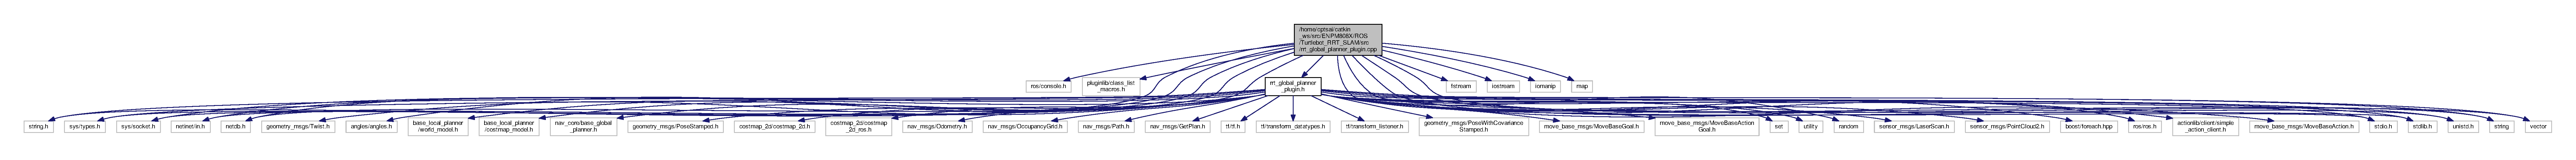
\includegraphics[width=350pt]{rrt__global__planner__plugin_8cpp__incl}
\end{center}
\end{figure}
\subsection*{Namespaces}
\begin{DoxyCompactItemize}
\item 
 \hyperlink{namespacerrt__planner}{rrt\+\_\+planner}
\end{DoxyCompactItemize}


\subsection{Detailed Description}
Implementation of rrt global planner. 

B\+SD License Copyright $<$2018$>$ $<$Chien-\/\+Te Lee$>$ $<$Chin-\/\+Po Tsai$>$

Redistribution and use in source and binary forms, with or without modification, are permitted provided that the following conditions are met\+:


\begin{DoxyEnumerate}
\item Redistributions of source code must retain the above copyright notice, this list of conditions and the following disclaimer.
\item Redistributions in binary form must reproduce the above copyright notice, this list of conditions and the following disclaimer in the documentation and/or other materials provided with the distribution.
\item Neither the name of the copyright holder nor the names of its contributors may be used to endorse or promote products derived from this software without specific prior written permission.
\end{DoxyEnumerate}

T\+H\+IS S\+O\+F\+T\+W\+A\+RE IS P\+R\+O\+V\+I\+D\+ED BY T\+HE C\+O\+P\+Y\+R\+I\+G\+HT H\+O\+L\+D\+E\+RS A\+ND C\+O\+N\+T\+R\+I\+B\+U\+T\+O\+RS \char`\"{}\+A\+S I\+S\char`\"{} A\+ND A\+NY E\+X\+P\+R\+E\+SS OR I\+M\+P\+L\+I\+ED W\+A\+R\+R\+A\+N\+T\+I\+ES, I\+N\+C\+L\+U\+D\+I\+NG, B\+UT N\+OT L\+I\+M\+I\+T\+ED TO, T\+HE I\+M\+P\+L\+I\+ED W\+A\+R\+R\+A\+N\+T\+I\+ES OF M\+E\+R\+C\+H\+A\+N\+T\+A\+B\+I\+L\+I\+TY A\+ND F\+I\+T\+N\+E\+SS F\+OR A P\+A\+R\+T\+I\+C\+U\+L\+AR P\+U\+R\+P\+O\+SE A\+RE D\+I\+S\+C\+L\+A\+I\+M\+ED. IN NO E\+V\+E\+NT S\+H\+A\+LL T\+HE C\+O\+P\+Y\+R\+I\+G\+HT H\+O\+L\+D\+ER OR C\+O\+N\+T\+R\+I\+B\+U\+T\+O\+RS BE L\+I\+A\+B\+LE F\+OR A\+NY D\+I\+R\+E\+CT, I\+N\+D\+I\+R\+E\+CT, I\+N\+C\+I\+D\+E\+N\+T\+AL, S\+P\+E\+C\+I\+AL, E\+X\+E\+M\+P\+L\+A\+RY, OR C\+O\+N\+S\+E\+Q\+U\+E\+N\+T\+I\+AL D\+A\+M\+A\+G\+ES (I\+N\+C\+L\+U\+D\+I\+NG, B\+UT N\+OT L\+I\+M\+I\+T\+ED TO, P\+R\+O\+C\+U\+R\+E\+M\+E\+NT OF S\+U\+B\+S\+T\+I\+T\+U\+TE G\+O\+O\+DS OR S\+E\+R\+V\+I\+C\+ES; L\+O\+SS OF U\+SE, D\+A\+TA, OR P\+R\+O\+F\+I\+TS; OR B\+U\+S\+I\+N\+E\+SS I\+N\+T\+E\+R\+R\+U\+P\+T\+I\+ON) H\+O\+W\+E\+V\+ER C\+A\+U\+S\+ED A\+ND ON A\+NY T\+H\+E\+O\+RY OF L\+I\+A\+B\+I\+L\+I\+TY, W\+H\+E\+T\+H\+ER IN C\+O\+N\+T\+R\+A\+CT, S\+T\+R\+I\+CT L\+I\+A\+B\+I\+L\+I\+TY, OR T\+O\+RT (I\+N\+C\+L\+U\+D\+I\+NG N\+E\+G\+L\+I\+G\+E\+N\+CE OR O\+T\+H\+E\+R\+W\+I\+SE) A\+R\+I\+S\+I\+NG IN A\+NY W\+AY O\+UT OF T\+HE U\+SE OF T\+H\+IS S\+O\+F\+T\+W\+A\+RE, E\+V\+EN IF A\+D\+V\+I\+S\+ED OF T\+HE P\+O\+S\+S\+I\+B\+I\+L\+I\+TY OF S\+U\+CH D\+A\+M\+A\+GE. \begin{DoxyCopyright}{Copyright}
(c) 2018 Chien-\/\+Te Lee, Chin-\/\+Po Tsai 
\end{DoxyCopyright}
\begin{DoxyAuthor}{Author}
Chien-\/\+Te Lee, Chin-\/\+Po Tsai 
\end{DoxyAuthor}
\begin{DoxyDate}{Date}
12/12/2018
\end{DoxyDate}
This file is applied as a plugin planner for R\+OS navigation stack. A R\+RT planner is implented under the global planner frame work 
\hypertarget{twist__to__wheel_8cpp}{}\section{/home/cptsai/catkin\+\_\+ws/src/\+E\+N\+P\+M808\+X/\+R\+O\+S/\+Turtlebot\+\_\+\+R\+R\+T\+\_\+\+S\+L\+A\+M/src/twist\+\_\+to\+\_\+wheel.cpp File Reference}
\label{twist__to__wheel_8cpp}\index{/home/cptsai/catkin\+\_\+ws/src/\+E\+N\+P\+M808\+X/\+R\+O\+S/\+Turtlebot\+\_\+\+R\+R\+T\+\_\+\+S\+L\+A\+M/src/twist\+\_\+to\+\_\+wheel.\+cpp@{/home/cptsai/catkin\+\_\+ws/src/\+E\+N\+P\+M808\+X/\+R\+O\+S/\+Turtlebot\+\_\+\+R\+R\+T\+\_\+\+S\+L\+A\+M/src/twist\+\_\+to\+\_\+wheel.\+cpp}}


Implementation of a subscriber for twist velocity topics.  


{\ttfamily \#include $<$twist\+\_\+to\+\_\+wheel.\+h$>$}\\*
{\ttfamily \#include $<$ros/ros.\+h$>$}\\*
{\ttfamily \#include $<$tf/transform\+\_\+listener.\+h$>$}\\*
{\ttfamily \#include $<$geometry\+\_\+msgs/\+Twist.\+h$>$}\\*
Include dependency graph for twist\+\_\+to\+\_\+wheel.\+cpp\+:
\nopagebreak
\begin{figure}[H]
\begin{center}
\leavevmode
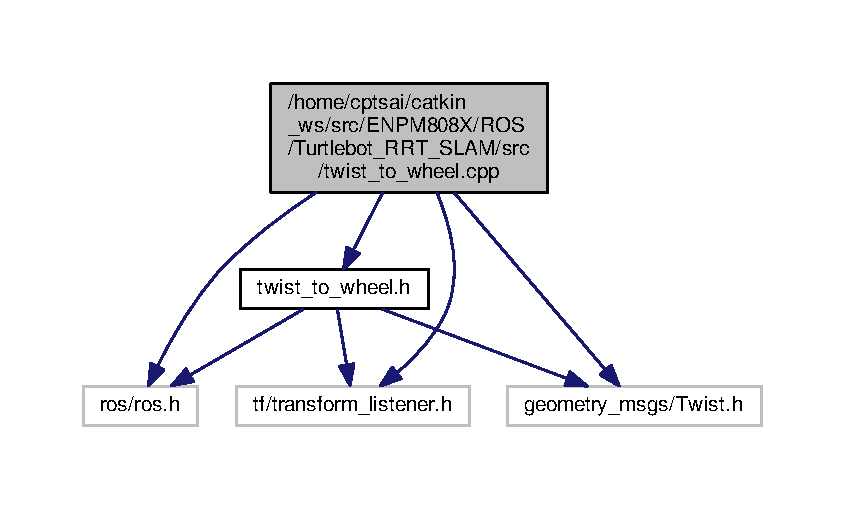
\includegraphics[width=350pt]{twist__to__wheel_8cpp__incl}
\end{center}
\end{figure}
\subsection*{Functions}
\begin{DoxyCompactItemize}
\item 
int \hyperlink{twist__to__wheel_8cpp_a3c04138a5bfe5d72780bb7e82a18e627}{main} (int argc, char $\ast$$\ast$argv)
\begin{DoxyCompactList}\small\item\em This function subscribes the velocity topics, and transform it to a motor velocity command in left/right wheel. \end{DoxyCompactList}\end{DoxyCompactItemize}


\subsection{Detailed Description}
Implementation of a subscriber for twist velocity topics. 

B\+SD License Copyright $<$2018$>$ $<$Chien-\/\+Te Lee$>$ $<$Chin-\/\+Po Tsai$>$

Redistribution and use in source and binary forms, with or without modification, are permitted provided that the following conditions are met\+:


\begin{DoxyEnumerate}
\item Redistributions of source code must retain the above copyright notice, this list of conditions and the following disclaimer.
\item Redistributions in binary form must reproduce the above copyright notice, this list of conditions and the following disclaimer in the documentation and/or other materials provided with the distribution.
\item Neither the name of the copyright holder nor the names of its contributors may be used to endorse or promote products derived from this software without specific prior written permission.
\end{DoxyEnumerate}

T\+H\+IS S\+O\+F\+T\+W\+A\+RE IS P\+R\+O\+V\+I\+D\+ED BY T\+HE C\+O\+P\+Y\+R\+I\+G\+HT H\+O\+L\+D\+E\+RS A\+ND C\+O\+N\+T\+R\+I\+B\+U\+T\+O\+RS \char`\"{}\+A\+S I\+S\char`\"{} A\+ND A\+NY E\+X\+P\+R\+E\+SS OR I\+M\+P\+L\+I\+ED W\+A\+R\+R\+A\+N\+T\+I\+ES, I\+N\+C\+L\+U\+D\+I\+NG, B\+UT N\+OT L\+I\+M\+I\+T\+ED TO, T\+HE I\+M\+P\+L\+I\+ED W\+A\+R\+R\+A\+N\+T\+I\+ES OF M\+E\+R\+C\+H\+A\+N\+T\+A\+B\+I\+L\+I\+TY A\+ND F\+I\+T\+N\+E\+SS F\+OR A P\+A\+R\+T\+I\+C\+U\+L\+AR P\+U\+R\+P\+O\+SE A\+RE D\+I\+S\+C\+L\+A\+I\+M\+ED. IN NO E\+V\+E\+NT S\+H\+A\+LL T\+HE C\+O\+P\+Y\+R\+I\+G\+HT H\+O\+L\+D\+ER OR C\+O\+N\+T\+R\+I\+B\+U\+T\+O\+RS BE L\+I\+A\+B\+LE F\+OR A\+NY D\+I\+R\+E\+CT, I\+N\+D\+I\+R\+E\+CT, I\+N\+C\+I\+D\+E\+N\+T\+AL, S\+P\+E\+C\+I\+AL, E\+X\+E\+M\+P\+L\+A\+RY, OR C\+O\+N\+S\+E\+Q\+U\+E\+N\+T\+I\+AL D\+A\+M\+A\+G\+ES (I\+N\+C\+L\+U\+D\+I\+NG, B\+UT N\+OT L\+I\+M\+I\+T\+ED TO, P\+R\+O\+C\+U\+R\+E\+M\+E\+NT OF S\+U\+B\+S\+T\+I\+T\+U\+TE G\+O\+O\+DS OR S\+E\+R\+V\+I\+C\+ES; L\+O\+SS OF U\+SE, D\+A\+TA, OR P\+R\+O\+F\+I\+TS; OR B\+U\+S\+I\+N\+E\+SS I\+N\+T\+E\+R\+R\+U\+P\+T\+I\+ON) H\+O\+W\+E\+V\+ER C\+A\+U\+S\+ED A\+ND ON A\+NY T\+H\+E\+O\+RY OF L\+I\+A\+B\+I\+L\+I\+TY, W\+H\+E\+T\+H\+ER IN C\+O\+N\+T\+R\+A\+CT, S\+T\+R\+I\+CT L\+I\+A\+B\+I\+L\+I\+TY, OR T\+O\+RT (I\+N\+C\+L\+U\+D\+I\+NG N\+E\+G\+L\+I\+G\+E\+N\+CE OR O\+T\+H\+E\+R\+W\+I\+SE) A\+R\+I\+S\+I\+NG IN A\+NY W\+AY O\+UT OF T\+HE U\+SE OF T\+H\+IS S\+O\+F\+T\+W\+A\+RE, E\+V\+EN IF A\+D\+V\+I\+S\+ED OF T\+HE P\+O\+S\+S\+I\+B\+I\+L\+I\+TY OF S\+U\+CH D\+A\+M\+A\+GE. \begin{DoxyCopyright}{Copyright}
(c) 2018 Chien-\/\+Te Lee, Chin-\/\+Po Tsai 
\end{DoxyCopyright}
\begin{DoxyAuthor}{Author}
Chien-\/\+Te Lee, Chin-\/\+Po Tsai 
\end{DoxyAuthor}
\begin{DoxyDate}{Date}
12/12/2018
\end{DoxyDate}
Implementation of a subscriber for twist velocity topics 

\subsection{Function Documentation}
\index{twist\+\_\+to\+\_\+wheel.\+cpp@{twist\+\_\+to\+\_\+wheel.\+cpp}!main@{main}}
\index{main@{main}!twist\+\_\+to\+\_\+wheel.\+cpp@{twist\+\_\+to\+\_\+wheel.\+cpp}}
\subsubsection[{\texorpdfstring{main(int argc, char $\ast$$\ast$argv)}{main(int argc, char **argv)}}]{\setlength{\rightskip}{0pt plus 5cm}int main (
\begin{DoxyParamCaption}
\item[{int}]{argc, }
\item[{char $\ast$$\ast$}]{argv}
\end{DoxyParamCaption}
)}\hypertarget{twist__to__wheel_8cpp_a3c04138a5bfe5d72780bb7e82a18e627}{}\label{twist__to__wheel_8cpp_a3c04138a5bfe5d72780bb7e82a18e627}


This function subscribes the velocity topics, and transform it to a motor velocity command in left/right wheel. 


\begin{DoxyParams}{Parameters}
{\em void} & \\
\hline
\end{DoxyParams}
\begin{DoxyReturn}{Returns}
int 
\end{DoxyReturn}

\hypertarget{test_8cpp}{}\section{/home/cptsai/catkin\+\_\+ws/src/\+E\+N\+P\+M808\+X/\+R\+O\+S/\+Turtlebot\+\_\+\+R\+R\+T\+\_\+\+S\+L\+A\+M/test/test.cpp File Reference}
\label{test_8cpp}\index{/home/cptsai/catkin\+\_\+ws/src/\+E\+N\+P\+M808\+X/\+R\+O\+S/\+Turtlebot\+\_\+\+R\+R\+T\+\_\+\+S\+L\+A\+M/test/test.\+cpp@{/home/cptsai/catkin\+\_\+ws/src/\+E\+N\+P\+M808\+X/\+R\+O\+S/\+Turtlebot\+\_\+\+R\+R\+T\+\_\+\+S\+L\+A\+M/test/test.\+cpp}}


Implementation of unit test for \hyperlink{namespacerrt__planner}{rrt\+\_\+planner} plugin.  


{\ttfamily \#include $<$rrt\+\_\+global\+\_\+planner\+\_\+plugin.\+h$>$}\\*
{\ttfamily \#include $<$twist\+\_\+to\+\_\+wheel.\+h$>$}\\*
{\ttfamily \#include $<$ros/ros.\+h$>$}\\*
{\ttfamily \#include $<$gtest/gtest.\+h$>$}\\*
Include dependency graph for test.\+cpp\+:
\nopagebreak
\begin{figure}[H]
\begin{center}
\leavevmode
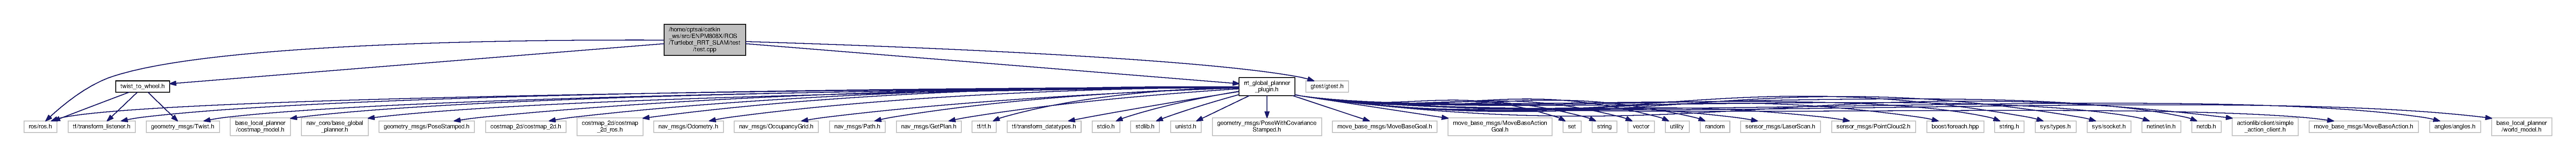
\includegraphics[width=350pt]{test_8cpp__incl}
\end{center}
\end{figure}
\subsection*{Functions}
\begin{DoxyCompactItemize}
\item 
\hyperlink{test_8cpp_a6ec787d9c7462529350c125ead3218bd}{T\+E\+ST} (T\+E\+S\+T\+Vertex, test\+Func1)
\begin{DoxyCompactList}\small\item\em $<$ ========== test vertex methods ==============// \end{DoxyCompactList}\item 
\hyperlink{test_8cpp_abc59086b38c8968e951857ea43fe6450}{T\+E\+ST} (T\+E\+S\+T\+Vertex, test\+Func2)
\begin{DoxyCompactList}\small\item\em This is a testcase for set\+Parent\+Idx() and get\+Parent\+Idx() \end{DoxyCompactList}\item 
\hyperlink{test_8cpp_ad50c366c8e8772ef98cb3f745a788d89}{T\+E\+ST} (T\+E\+S\+T\+Vertex, test\+Func3)
\begin{DoxyCompactList}\small\item\em This is a testcase for set\+Idx() and get\+Idx() \end{DoxyCompactList}\item 
\hyperlink{test_8cpp_afba96da4893441721b87e71d8e82c669}{T\+E\+ST} (T\+E\+S\+T\+R\+R\+Tplanner, test\+Func1)
\begin{DoxyCompactList}\small\item\em This is a testcase for get\+Cell\+Index() \end{DoxyCompactList}\item 
\hyperlink{test_8cpp_a3ef17c0493415d4bf1d3dc5dcbc71500}{T\+E\+ST} (T\+E\+S\+T\+R\+R\+Tplanner, test\+Func2)
\begin{DoxyCompactList}\small\item\em This is a testcase for get\+Cell\+Row\+I\+D() \end{DoxyCompactList}\item 
\hyperlink{test_8cpp_a7ab65bc636fe161556e7de401c0279dd}{T\+E\+ST} (T\+E\+S\+T\+R\+R\+Tplanner, test\+Func3)
\begin{DoxyCompactList}\small\item\em This is a testcase for get\+Cell\+Col\+I\+D() \end{DoxyCompactList}\item 
\hyperlink{test_8cpp_a59e8e3c15b3e80b5aa31c54ea75a4589}{T\+E\+ST} (T\+E\+S\+T\+R\+R\+Tplanner, test\+Func4)
\begin{DoxyCompactList}\small\item\em This is a testcase for get\+Corrdinate() \end{DoxyCompactList}\item 
\hyperlink{test_8cpp_aecdcee1c5f30082ebbf27bb13e2dc7fb}{T\+E\+ST} (T\+E\+S\+T\+R\+R\+Tplanner, test\+Func5)
\begin{DoxyCompactList}\small\item\em This is a testcase for convert\+To\+Cell\+Index() \end{DoxyCompactList}\item 
\hyperlink{test_8cpp_ad3f2ec6e2929a51995ca77affecba969}{T\+E\+ST} (T\+E\+S\+T\+R\+R\+Tplanner, test\+Func6)
\begin{DoxyCompactList}\small\item\em This is a testcase for convert\+To\+Coordinate() \end{DoxyCompactList}\item 
\hyperlink{test_8cpp_a7caf067ee6e947f57c6ade24ecce4e7b}{T\+E\+ST} (T\+E\+S\+T\+R\+R\+Tplanner, test\+Func7)
\begin{DoxyCompactList}\small\item\em This is a testcase for is\+Cell\+Inside\+Map() \end{DoxyCompactList}\item 
\hyperlink{test_8cpp_ac1dcae23b2e4a9bd6794a1a28d0c106a}{T\+E\+ST} (T\+E\+S\+T\+R\+R\+Tplanner, test\+Func8)
\begin{DoxyCompactList}\small\item\em This is a testcase for Get\+Random\+Point() \end{DoxyCompactList}\item 
\hyperlink{test_8cpp_a14a83a4efade5aaf246ed76621435984}{T\+E\+ST} (T\+E\+S\+T\+R\+R\+Tplanner, test\+Func9)
\begin{DoxyCompactList}\small\item\em This is a testcase for is\+Free() \end{DoxyCompactList}\item 
\hyperlink{test_8cpp_a365aa4a86314d6e3cad85c04b6faa459}{T\+E\+ST} (T\+E\+S\+T\+R\+R\+Tplanner, test\+Func10)
\begin{DoxyCompactList}\small\item\em This is a testcase for is\+Free() \end{DoxyCompactList}\item 
\hyperlink{test_8cpp_a46815c7a9ebe47516cd17a5479d268a4}{T\+E\+ST} (T\+E\+S\+T\+R\+R\+Tplanner, test\+Func11)
\begin{DoxyCompactList}\small\item\em This is a testcase for is\+Start\+And\+Goal\+Cells\+Valid() \end{DoxyCompactList}\item 
\hyperlink{test_8cpp_a0a60afc7d7c45638769d2bf83e2aa3de}{T\+E\+ST} (T\+E\+S\+T\+R\+R\+Tplanner, test\+Func12)
\begin{DoxyCompactList}\small\item\em This is a testcase for rrt\+Planner() \end{DoxyCompactList}\item 
\hyperlink{test_8cpp_a05d10c5f97ef11d69a6bce47cbdacb0b}{T\+E\+ST} (T\+E\+S\+T\+Subscriber\+Callback, test\+Twist\+Cb)
\begin{DoxyCompactList}\small\item\em This is a testcase for subscriber callback funciton. \end{DoxyCompactList}\item 
int \hyperlink{test_8cpp_a3c04138a5bfe5d72780bb7e82a18e627}{main} (int argc, char $\ast$$\ast$argv)
\begin{DoxyCompactList}\small\item\em main fucntion to run all testcases \end{DoxyCompactList}\end{DoxyCompactItemize}


\subsection{Detailed Description}
Implementation of unit test for \hyperlink{namespacerrt__planner}{rrt\+\_\+planner} plugin. 

B\+SD 3 clauses Liscense

Copyright $<$2018$>$ $<$Chien-\/\+Te Lee$>$ $<$Chin-\/\+Po Tsai$>$

Redistribution and use in source and binary forms, with or without modification, are permitted provided that the following conditions are met\+:


\begin{DoxyEnumerate}
\item Redistributions of source code must retain the above copyright notice, this list of conditions and the following disclaimer.
\item Redistributions in binary form must reproduce the above copyright notice, this list of conditions and the following disclaimer in the documentation and/or other materials provided with the distribution.
\item Neither the name of the copyright holder nor the names of its contributors may be used to endorse or promote products derived from this software without specific prior written permission.
\end{DoxyEnumerate}

T\+H\+IS S\+O\+F\+T\+W\+A\+RE IS P\+R\+O\+V\+I\+D\+ED BY T\+HE C\+O\+P\+Y\+R\+I\+G\+HT H\+O\+L\+D\+E\+RS A\+ND C\+O\+N\+T\+R\+I\+B\+U\+T\+O\+RS \char`\"{}\+A\+S I\+S\char`\"{} A\+ND A\+NY E\+X\+P\+R\+E\+SS OR I\+M\+P\+L\+I\+ED W\+A\+R\+R\+A\+N\+T\+I\+ES, I\+N\+C\+L\+U\+D\+I\+NG, B\+UT N\+OT L\+I\+M\+I\+T\+ED TO, T\+HE I\+M\+P\+L\+I\+ED W\+A\+R\+R\+A\+N\+T\+I\+ES OF M\+E\+R\+C\+H\+A\+N\+T\+A\+B\+I\+L\+I\+TY A\+ND F\+I\+T\+N\+E\+SS F\+OR A P\+A\+R\+T\+I\+C\+U\+L\+AR P\+U\+R\+P\+O\+SE A\+RE D\+I\+S\+C\+L\+A\+I\+M\+ED. IN NO E\+V\+E\+NT S\+H\+A\+LL T\+HE C\+O\+P\+Y\+R\+I\+G\+HT H\+O\+L\+D\+ER OR C\+O\+N\+T\+R\+I\+B\+U\+T\+O\+RS BE L\+I\+A\+B\+LE F\+OR A\+NY D\+I\+R\+E\+CT, I\+N\+D\+I\+R\+E\+CT, I\+N\+C\+I\+D\+E\+N\+T\+AL, S\+P\+E\+C\+I\+AL, E\+X\+E\+M\+P\+L\+A\+RY, OR C\+O\+N\+S\+E\+Q\+U\+E\+N\+T\+I\+AL D\+A\+M\+A\+G\+ES (I\+N\+C\+L\+U\+D\+I\+NG, B\+UT N\+OT L\+I\+M\+I\+T\+ED TO, P\+R\+O\+C\+U\+R\+E\+M\+E\+NT OF S\+U\+B\+S\+T\+I\+T\+U\+TE G\+O\+O\+DS OR S\+E\+R\+V\+I\+C\+ES; L\+O\+SS OF U\+SE, D\+A\+TA, OR P\+R\+O\+F\+I\+TS; OR B\+U\+S\+I\+N\+E\+SS I\+N\+T\+E\+R\+R\+U\+P\+T\+I\+ON) H\+O\+W\+E\+V\+ER C\+A\+U\+S\+ED A\+ND ON A\+NY T\+H\+E\+O\+RY OF L\+I\+A\+B\+I\+L\+I\+TY, W\+H\+E\+T\+H\+ER IN C\+O\+N\+T\+R\+A\+CT, S\+T\+R\+I\+CT L\+I\+A\+B\+I\+L\+I\+TY, OR T\+O\+RT (I\+N\+C\+L\+U\+D\+I\+NG N\+E\+G\+L\+I\+G\+E\+N\+CE OR O\+T\+H\+E\+R\+W\+I\+SE) A\+R\+I\+S\+I\+NG IN A\+NY W\+AY O\+UT OF T\+HE U\+SE OF T\+H\+IS S\+O\+F\+T\+W\+A\+RE, E\+V\+EN IF A\+D\+V\+I\+S\+ED OF T\+HE P\+O\+S\+S\+I\+B\+I\+L\+I\+TY OF S\+U\+CH D\+A\+M\+A\+GE. \begin{DoxyCopyright}{Copyright}
(c) 2018 Chien-\/\+Te Lee, Chin-\/\+Po Tsai 
\end{DoxyCopyright}
\begin{DoxyAuthor}{Author}
Chien-\/\+Te Lee, Chin-\/\+Po Tsai 
\end{DoxyAuthor}
\begin{DoxyDate}{Date}
12/16/2018
\end{DoxyDate}
This program implemnts unit test for methods of class vertex and rrt\+Planner\+R\+OS, and subscriber callback function of twist\+\_\+to\+\_\+wheel. 

\subsection{Function Documentation}
\index{test.\+cpp@{test.\+cpp}!main@{main}}
\index{main@{main}!test.\+cpp@{test.\+cpp}}
\subsubsection[{\texorpdfstring{main(int argc, char $\ast$$\ast$argv)}{main(int argc, char **argv)}}]{\setlength{\rightskip}{0pt plus 5cm}int main (
\begin{DoxyParamCaption}
\item[{int}]{argc, }
\item[{char $\ast$$\ast$}]{argv}
\end{DoxyParamCaption}
)}\hypertarget{test_8cpp_a3c04138a5bfe5d72780bb7e82a18e627}{}\label{test_8cpp_a3c04138a5bfe5d72780bb7e82a18e627}


main fucntion to run all testcases 


\begin{DoxyParams}{Parameters}
{\em argc} & is the number of input argument \\
\hline
{\em argv} & are the input arguments \\
\hline
\end{DoxyParams}
\begin{DoxyReturn}{Returns}
0 if all the tests are successful 
\end{DoxyReturn}
\index{test.\+cpp@{test.\+cpp}!T\+E\+ST@{T\+E\+ST}}
\index{T\+E\+ST@{T\+E\+ST}!test.\+cpp@{test.\+cpp}}
\subsubsection[{\texorpdfstring{T\+E\+S\+T(\+T\+E\+S\+T\+Vertex, test\+Func1)}{TEST(TESTVertex, testFunc1)}}]{\setlength{\rightskip}{0pt plus 5cm}T\+E\+ST (
\begin{DoxyParamCaption}
\item[{T\+E\+S\+T\+Vertex}]{, }
\item[{test\+Func1}]{}
\end{DoxyParamCaption}
)}\hypertarget{test_8cpp_a6ec787d9c7462529350c125ead3218bd}{}\label{test_8cpp_a6ec787d9c7462529350c125ead3218bd}


$<$ ========== test vertex methods ==============// 

This is a testcase for set\+Position() and get\+Position() 
\begin{DoxyParams}{Parameters}
{\em T\+E\+S\+T\+Vertex} & is the name of the test suite \\
\hline
{\em test\+Func1} & is the name of the testcase \\
\hline
\end{DoxyParams}
\begin{DoxyReturn}{Returns}
none 
\end{DoxyReturn}
\index{test.\+cpp@{test.\+cpp}!T\+E\+ST@{T\+E\+ST}}
\index{T\+E\+ST@{T\+E\+ST}!test.\+cpp@{test.\+cpp}}
\subsubsection[{\texorpdfstring{T\+E\+S\+T(\+T\+E\+S\+T\+Vertex, test\+Func2)}{TEST(TESTVertex, testFunc2)}}]{\setlength{\rightskip}{0pt plus 5cm}T\+E\+ST (
\begin{DoxyParamCaption}
\item[{T\+E\+S\+T\+Vertex}]{, }
\item[{test\+Func2}]{}
\end{DoxyParamCaption}
)}\hypertarget{test_8cpp_abc59086b38c8968e951857ea43fe6450}{}\label{test_8cpp_abc59086b38c8968e951857ea43fe6450}


This is a testcase for set\+Parent\+Idx() and get\+Parent\+Idx() 


\begin{DoxyParams}{Parameters}
{\em T\+E\+S\+T\+Vertex} & is the name of the test suite \\
\hline
{\em test\+Func2} & is the name of the testcase \\
\hline
\end{DoxyParams}
\begin{DoxyReturn}{Returns}
none 
\end{DoxyReturn}
\index{test.\+cpp@{test.\+cpp}!T\+E\+ST@{T\+E\+ST}}
\index{T\+E\+ST@{T\+E\+ST}!test.\+cpp@{test.\+cpp}}
\subsubsection[{\texorpdfstring{T\+E\+S\+T(\+T\+E\+S\+T\+Vertex, test\+Func3)}{TEST(TESTVertex, testFunc3)}}]{\setlength{\rightskip}{0pt plus 5cm}T\+E\+ST (
\begin{DoxyParamCaption}
\item[{T\+E\+S\+T\+Vertex}]{, }
\item[{test\+Func3}]{}
\end{DoxyParamCaption}
)}\hypertarget{test_8cpp_ad50c366c8e8772ef98cb3f745a788d89}{}\label{test_8cpp_ad50c366c8e8772ef98cb3f745a788d89}


This is a testcase for set\+Idx() and get\+Idx() 


\begin{DoxyParams}{Parameters}
{\em T\+E\+S\+T\+Vertex} & is the name of the test suite \\
\hline
{\em test\+Func3} & is the name of the testcase \\
\hline
\end{DoxyParams}
\begin{DoxyReturn}{Returns}
none 
\end{DoxyReturn}
\index{test.\+cpp@{test.\+cpp}!T\+E\+ST@{T\+E\+ST}}
\index{T\+E\+ST@{T\+E\+ST}!test.\+cpp@{test.\+cpp}}
\subsubsection[{\texorpdfstring{T\+E\+S\+T(\+T\+E\+S\+T\+R\+R\+Tplanner, test\+Func1)}{TEST(TESTRRTplanner, testFunc1)}}]{\setlength{\rightskip}{0pt plus 5cm}T\+E\+ST (
\begin{DoxyParamCaption}
\item[{T\+E\+S\+T\+R\+R\+Tplanner}]{, }
\item[{test\+Func1}]{}
\end{DoxyParamCaption}
)}\hypertarget{test_8cpp_afba96da4893441721b87e71d8e82c669}{}\label{test_8cpp_afba96da4893441721b87e71d8e82c669}


This is a testcase for get\+Cell\+Index() 


\begin{DoxyParams}{Parameters}
{\em T\+E\+S\+T\+R\+R\+Tplanner} & is the name of the test suite \\
\hline
{\em test\+Func1} & is the name of the testcase \\
\hline
\end{DoxyParams}
\begin{DoxyReturn}{Returns}
none 
\end{DoxyReturn}
\index{test.\+cpp@{test.\+cpp}!T\+E\+ST@{T\+E\+ST}}
\index{T\+E\+ST@{T\+E\+ST}!test.\+cpp@{test.\+cpp}}
\subsubsection[{\texorpdfstring{T\+E\+S\+T(\+T\+E\+S\+T\+R\+R\+Tplanner, test\+Func2)}{TEST(TESTRRTplanner, testFunc2)}}]{\setlength{\rightskip}{0pt plus 5cm}T\+E\+ST (
\begin{DoxyParamCaption}
\item[{T\+E\+S\+T\+R\+R\+Tplanner}]{, }
\item[{test\+Func2}]{}
\end{DoxyParamCaption}
)}\hypertarget{test_8cpp_a3ef17c0493415d4bf1d3dc5dcbc71500}{}\label{test_8cpp_a3ef17c0493415d4bf1d3dc5dcbc71500}


This is a testcase for get\+Cell\+Row\+I\+D() 


\begin{DoxyParams}{Parameters}
{\em T\+E\+S\+T\+R\+R\+Tplanner} & is the name of the test suite \\
\hline
{\em test\+Func2} & is the name of the testcase \\
\hline
\end{DoxyParams}
\begin{DoxyReturn}{Returns}
none 
\end{DoxyReturn}
\index{test.\+cpp@{test.\+cpp}!T\+E\+ST@{T\+E\+ST}}
\index{T\+E\+ST@{T\+E\+ST}!test.\+cpp@{test.\+cpp}}
\subsubsection[{\texorpdfstring{T\+E\+S\+T(\+T\+E\+S\+T\+R\+R\+Tplanner, test\+Func3)}{TEST(TESTRRTplanner, testFunc3)}}]{\setlength{\rightskip}{0pt plus 5cm}T\+E\+ST (
\begin{DoxyParamCaption}
\item[{T\+E\+S\+T\+R\+R\+Tplanner}]{, }
\item[{test\+Func3}]{}
\end{DoxyParamCaption}
)}\hypertarget{test_8cpp_a7ab65bc636fe161556e7de401c0279dd}{}\label{test_8cpp_a7ab65bc636fe161556e7de401c0279dd}


This is a testcase for get\+Cell\+Col\+I\+D() 


\begin{DoxyParams}{Parameters}
{\em T\+E\+S\+T\+R\+R\+Tplanner} & is the name of the test suite \\
\hline
{\em test\+Func3} & is the name of the testcase \\
\hline
\end{DoxyParams}
\begin{DoxyReturn}{Returns}
none 
\end{DoxyReturn}
\index{test.\+cpp@{test.\+cpp}!T\+E\+ST@{T\+E\+ST}}
\index{T\+E\+ST@{T\+E\+ST}!test.\+cpp@{test.\+cpp}}
\subsubsection[{\texorpdfstring{T\+E\+S\+T(\+T\+E\+S\+T\+R\+R\+Tplanner, test\+Func4)}{TEST(TESTRRTplanner, testFunc4)}}]{\setlength{\rightskip}{0pt plus 5cm}T\+E\+ST (
\begin{DoxyParamCaption}
\item[{T\+E\+S\+T\+R\+R\+Tplanner}]{, }
\item[{test\+Func4}]{}
\end{DoxyParamCaption}
)}\hypertarget{test_8cpp_a59e8e3c15b3e80b5aa31c54ea75a4589}{}\label{test_8cpp_a59e8e3c15b3e80b5aa31c54ea75a4589}


This is a testcase for get\+Corrdinate() 


\begin{DoxyParams}{Parameters}
{\em T\+E\+S\+T\+R\+R\+Tplanner} & is the name of the test suite \\
\hline
{\em test\+Func4} & is the name of the testcase \\
\hline
\end{DoxyParams}
\begin{DoxyReturn}{Returns}
none 
\end{DoxyReturn}
\index{test.\+cpp@{test.\+cpp}!T\+E\+ST@{T\+E\+ST}}
\index{T\+E\+ST@{T\+E\+ST}!test.\+cpp@{test.\+cpp}}
\subsubsection[{\texorpdfstring{T\+E\+S\+T(\+T\+E\+S\+T\+R\+R\+Tplanner, test\+Func5)}{TEST(TESTRRTplanner, testFunc5)}}]{\setlength{\rightskip}{0pt plus 5cm}T\+E\+ST (
\begin{DoxyParamCaption}
\item[{T\+E\+S\+T\+R\+R\+Tplanner}]{, }
\item[{test\+Func5}]{}
\end{DoxyParamCaption}
)}\hypertarget{test_8cpp_aecdcee1c5f30082ebbf27bb13e2dc7fb}{}\label{test_8cpp_aecdcee1c5f30082ebbf27bb13e2dc7fb}


This is a testcase for convert\+To\+Cell\+Index() 


\begin{DoxyParams}{Parameters}
{\em T\+E\+S\+T\+R\+R\+Tplanner} & is the name of the test suite \\
\hline
{\em test\+Func5} & is the name of the testcase \\
\hline
\end{DoxyParams}
\begin{DoxyReturn}{Returns}
none 
\end{DoxyReturn}
\index{test.\+cpp@{test.\+cpp}!T\+E\+ST@{T\+E\+ST}}
\index{T\+E\+ST@{T\+E\+ST}!test.\+cpp@{test.\+cpp}}
\subsubsection[{\texorpdfstring{T\+E\+S\+T(\+T\+E\+S\+T\+R\+R\+Tplanner, test\+Func6)}{TEST(TESTRRTplanner, testFunc6)}}]{\setlength{\rightskip}{0pt plus 5cm}T\+E\+ST (
\begin{DoxyParamCaption}
\item[{T\+E\+S\+T\+R\+R\+Tplanner}]{, }
\item[{test\+Func6}]{}
\end{DoxyParamCaption}
)}\hypertarget{test_8cpp_ad3f2ec6e2929a51995ca77affecba969}{}\label{test_8cpp_ad3f2ec6e2929a51995ca77affecba969}


This is a testcase for convert\+To\+Coordinate() 


\begin{DoxyParams}{Parameters}
{\em T\+E\+S\+T\+R\+R\+Tplanner} & is the name of the test suite \\
\hline
{\em test\+Func6} & is the name of the testcase \\
\hline
\end{DoxyParams}
\begin{DoxyReturn}{Returns}
none 
\end{DoxyReturn}
\index{test.\+cpp@{test.\+cpp}!T\+E\+ST@{T\+E\+ST}}
\index{T\+E\+ST@{T\+E\+ST}!test.\+cpp@{test.\+cpp}}
\subsubsection[{\texorpdfstring{T\+E\+S\+T(\+T\+E\+S\+T\+R\+R\+Tplanner, test\+Func7)}{TEST(TESTRRTplanner, testFunc7)}}]{\setlength{\rightskip}{0pt plus 5cm}T\+E\+ST (
\begin{DoxyParamCaption}
\item[{T\+E\+S\+T\+R\+R\+Tplanner}]{, }
\item[{test\+Func7}]{}
\end{DoxyParamCaption}
)}\hypertarget{test_8cpp_a7caf067ee6e947f57c6ade24ecce4e7b}{}\label{test_8cpp_a7caf067ee6e947f57c6ade24ecce4e7b}


This is a testcase for is\+Cell\+Inside\+Map() 


\begin{DoxyParams}{Parameters}
{\em T\+E\+S\+T\+R\+R\+Tplanner} & is the name of the test suite \\
\hline
{\em test\+Func7} & is the name of the testcase \\
\hline
\end{DoxyParams}
\begin{DoxyReturn}{Returns}
none 
\end{DoxyReturn}
\index{test.\+cpp@{test.\+cpp}!T\+E\+ST@{T\+E\+ST}}
\index{T\+E\+ST@{T\+E\+ST}!test.\+cpp@{test.\+cpp}}
\subsubsection[{\texorpdfstring{T\+E\+S\+T(\+T\+E\+S\+T\+R\+R\+Tplanner, test\+Func8)}{TEST(TESTRRTplanner, testFunc8)}}]{\setlength{\rightskip}{0pt plus 5cm}T\+E\+ST (
\begin{DoxyParamCaption}
\item[{T\+E\+S\+T\+R\+R\+Tplanner}]{, }
\item[{test\+Func8}]{}
\end{DoxyParamCaption}
)}\hypertarget{test_8cpp_ac1dcae23b2e4a9bd6794a1a28d0c106a}{}\label{test_8cpp_ac1dcae23b2e4a9bd6794a1a28d0c106a}


This is a testcase for Get\+Random\+Point() 


\begin{DoxyParams}{Parameters}
{\em T\+E\+S\+T\+R\+R\+Tplanner} & is the name of the test suite \\
\hline
{\em test\+Func8} & is the name of the testcase \\
\hline
\end{DoxyParams}
\begin{DoxyReturn}{Returns}
none 
\end{DoxyReturn}
\index{test.\+cpp@{test.\+cpp}!T\+E\+ST@{T\+E\+ST}}
\index{T\+E\+ST@{T\+E\+ST}!test.\+cpp@{test.\+cpp}}
\subsubsection[{\texorpdfstring{T\+E\+S\+T(\+T\+E\+S\+T\+R\+R\+Tplanner, test\+Func9)}{TEST(TESTRRTplanner, testFunc9)}}]{\setlength{\rightskip}{0pt plus 5cm}T\+E\+ST (
\begin{DoxyParamCaption}
\item[{T\+E\+S\+T\+R\+R\+Tplanner}]{, }
\item[{test\+Func9}]{}
\end{DoxyParamCaption}
)}\hypertarget{test_8cpp_a14a83a4efade5aaf246ed76621435984}{}\label{test_8cpp_a14a83a4efade5aaf246ed76621435984}


This is a testcase for is\+Free() 


\begin{DoxyParams}{Parameters}
{\em T\+E\+S\+T\+R\+R\+Tplanner} & is the name of the test suite \\
\hline
{\em test\+Func9} & is the name of the testcase \\
\hline
\end{DoxyParams}
\begin{DoxyReturn}{Returns}
none 
\end{DoxyReturn}
\index{test.\+cpp@{test.\+cpp}!T\+E\+ST@{T\+E\+ST}}
\index{T\+E\+ST@{T\+E\+ST}!test.\+cpp@{test.\+cpp}}
\subsubsection[{\texorpdfstring{T\+E\+S\+T(\+T\+E\+S\+T\+R\+R\+Tplanner, test\+Func10)}{TEST(TESTRRTplanner, testFunc10)}}]{\setlength{\rightskip}{0pt plus 5cm}T\+E\+ST (
\begin{DoxyParamCaption}
\item[{T\+E\+S\+T\+R\+R\+Tplanner}]{, }
\item[{test\+Func10}]{}
\end{DoxyParamCaption}
)}\hypertarget{test_8cpp_a365aa4a86314d6e3cad85c04b6faa459}{}\label{test_8cpp_a365aa4a86314d6e3cad85c04b6faa459}


This is a testcase for is\+Free() 


\begin{DoxyParams}{Parameters}
{\em T\+E\+S\+T\+R\+R\+Tplanner} & is the name of the test suite \\
\hline
{\em test\+Func10} & is the name of the testcase \\
\hline
\end{DoxyParams}
\begin{DoxyReturn}{Returns}
none 
\end{DoxyReturn}
\index{test.\+cpp@{test.\+cpp}!T\+E\+ST@{T\+E\+ST}}
\index{T\+E\+ST@{T\+E\+ST}!test.\+cpp@{test.\+cpp}}
\subsubsection[{\texorpdfstring{T\+E\+S\+T(\+T\+E\+S\+T\+R\+R\+Tplanner, test\+Func11)}{TEST(TESTRRTplanner, testFunc11)}}]{\setlength{\rightskip}{0pt plus 5cm}T\+E\+ST (
\begin{DoxyParamCaption}
\item[{T\+E\+S\+T\+R\+R\+Tplanner}]{, }
\item[{test\+Func11}]{}
\end{DoxyParamCaption}
)}\hypertarget{test_8cpp_a46815c7a9ebe47516cd17a5479d268a4}{}\label{test_8cpp_a46815c7a9ebe47516cd17a5479d268a4}


This is a testcase for is\+Start\+And\+Goal\+Cells\+Valid() 


\begin{DoxyParams}{Parameters}
{\em T\+E\+S\+T\+R\+R\+Tplanner} & is the name of the test suite \\
\hline
{\em test\+Func11} & is the name of the testcase \\
\hline
\end{DoxyParams}
\begin{DoxyReturn}{Returns}
none 
\end{DoxyReturn}
\index{test.\+cpp@{test.\+cpp}!T\+E\+ST@{T\+E\+ST}}
\index{T\+E\+ST@{T\+E\+ST}!test.\+cpp@{test.\+cpp}}
\subsubsection[{\texorpdfstring{T\+E\+S\+T(\+T\+E\+S\+T\+R\+R\+Tplanner, test\+Func12)}{TEST(TESTRRTplanner, testFunc12)}}]{\setlength{\rightskip}{0pt plus 5cm}T\+E\+ST (
\begin{DoxyParamCaption}
\item[{T\+E\+S\+T\+R\+R\+Tplanner}]{, }
\item[{test\+Func12}]{}
\end{DoxyParamCaption}
)}\hypertarget{test_8cpp_a0a60afc7d7c45638769d2bf83e2aa3de}{}\label{test_8cpp_a0a60afc7d7c45638769d2bf83e2aa3de}


This is a testcase for rrt\+Planner() 


\begin{DoxyParams}{Parameters}
{\em T\+E\+S\+T\+R\+R\+Tplanner} & is the name of the test suite \\
\hline
{\em test\+Func12} & is the name of the testcase \\
\hline
\end{DoxyParams}
\begin{DoxyReturn}{Returns}
none 
\end{DoxyReturn}
\index{test.\+cpp@{test.\+cpp}!T\+E\+ST@{T\+E\+ST}}
\index{T\+E\+ST@{T\+E\+ST}!test.\+cpp@{test.\+cpp}}
\subsubsection[{\texorpdfstring{T\+E\+S\+T(\+T\+E\+S\+T\+Subscriber\+Callback, test\+Twist\+Cb)}{TEST(TESTSubscriberCallback, testTwistCb)}}]{\setlength{\rightskip}{0pt plus 5cm}T\+E\+ST (
\begin{DoxyParamCaption}
\item[{T\+E\+S\+T\+Subscriber\+Callback}]{, }
\item[{test\+Twist\+Cb}]{}
\end{DoxyParamCaption}
)}\hypertarget{test_8cpp_a05d10c5f97ef11d69a6bce47cbdacb0b}{}\label{test_8cpp_a05d10c5f97ef11d69a6bce47cbdacb0b}


This is a testcase for subscriber callback funciton. 


\begin{DoxyParams}{Parameters}
{\em T\+E\+S\+T\+Subscriber\+Callback} & is the name of the test suite \\
\hline
{\em test\+Twist\+Cb} & is the name of the testcase \\
\hline
\end{DoxyParams}
\begin{DoxyReturn}{Returns}
none 
\end{DoxyReturn}
$<$ run publisher and check publisher and subscriber

$<$ run subscriber and check publisher and subscriber 
%--- End generated contents ---

% Index
\backmatter
\newpage
\phantomsection
\clearemptydoublepage
\addcontentsline{toc}{chapter}{Index}
\printindex

\end{document}
